\documentclass[12pt]{report}

\def\magyarOptions{defaults=hu-min}
\usepackage[magyar]{babel}
\usepackage[utf8]{inputenc}
\usepackage{t1enc}

\usepackage{times}

\usepackage{amsmath}
\usepackage{amssymb}
\usepackage{amsthm}

\usepackage{graphicx}
\graphicspath{{figures/}}

\usepackage[bottom,hang,flushmargin]{footmisc}
\usepackage[many]{tcolorbox}

\usepackage{enumitem}
\usepackage{fancyhdr}
\usepackage{float}
\usepackage{hyperref}
\usepackage{makecell}
\usepackage{verbatim}
\usepackage{xcolor}

\usepackage{listings}
\lstset{
    basicstyle=\ttfamily\small,
    rulecolor=\color{gray},
    frame=b,
}

\usepackage{caption}
\DeclareCaptionFont{white}{\color{white}}
\DeclareCaptionFormat{listing}{\colorbox{gray}{\parbox{148mm}{\bfseries#3}}}
\captionsetup[lstlisting]{format=listing,labelfont=white,textfont=white}


% Margins
\hoffset -1in
\voffset -1in
\oddsidemargin 35mm
\textwidth 150mm
\topmargin 15mm
\headheight 10mm
\headsep 5mm
\textheight 237mm

% Justification
\tolerance=1
\emergencystretch=\maxdimen
\hyphenpenalty=10000
\hbadness=10000
\sloppy

% Colors
\definecolor{qtgreen}{HTML}{44A51C}
\definecolor{qtred}{HTML}{A5441C}

% URL style
\hypersetup{
    colorlinks=false, % Disable colorlinks for not coloring table of contents
    unicode=true,
}

\let\orighref\href
\renewcommand{\href}[2]{%
    \orighref{#1}{\textcolor{blue}{\texttt{#2}}}
}

\let\origurl\url
\renewcommand{\url}[1]{%
    \textcolor{blue}{\origurl{#1}}
}

\newcommand{\todo}[1]{%
    \textcolor{red}{\textbf{TODO:} #1}
}

\newcommand{\fixme}[1]{%
    \textcolor{red}{\textbf{FIXME:} #1}
}

\newcommand{\gerrit}[1]{%
    \textcolor{qtgreen}{\origurl{https://codereview.qt-project.org/\#/c/#1}}
}

\newcommand{\qtbug}[1]{%
    \textcolor{qtred}{\origurl{https://bugreports.qt.io/browse/QTBUG-#1}}
}

\setdescription{
    style=standard,
    align=right,
    itemindent=1cm,
    labelwidth=1cm,
    leftmargin=1cm,
    before={\renewcommand\makelabel[1]{\bfseries ########1:}},
    %font=\sffamily\bfseries,
}

\newtcolorbox{reviewbox}[1][]
  {title=Gerrit Code Review,
   width=12.5cm,
   left=0pt,
   right=0pt,
   fonttitle=\bfseries,
   coltitle=white,
   colframe=qtgreen,
   colback=white,
   #1
}

\newtcolorbox{issuebox}[1][]
  {title=Jira Issue,
   width=12.5cm,
   left=0pt,
   right=0pt,
   fonttitle=\bfseries,
   coltitle=white,
   colframe=qtred,
   colback=white,
   #1
}


\hyphenation{QtWebEngine QtWebKit WebKit Chromium Content Apple Google Quick Widget WebSocket
QtWebSockets QtWebChannel Android WebEngine JavaScript JavaScriptCore WebCore thread}

\def\title{A QtWebEngine bővítése és bemutatása saját böngészőalkalmazás segítségével}

\begin{document}

% EMPTY PAGE STYLE
\fancypagestyle{plain}{
    \fancyhf{}
    \fancyfoot[R]{\thepage}
    \renewcommand{\headrulewidth}{0pt}
}

% FOOTER & HEADER
\pagestyle{fancy}
\fancyhf{}
\fancyhead[L]{\title}
\fancyfoot[R]{\thepage}
%\fancyfoot[C]{\thepage}

%%% TITLE PAGE %%%
\thispagestyle{empty}
\begin{center}
    \vspace*{1cm}
    {\Large\textbf{Szegedi Tudományegyetem}}

    \vspace{0.5cm}
    {\Large\textbf{Informatikai Tanszékcsoport}}

    \vspace{3.8cm}
    {\LARGE\textbf{\title}}

    \vspace{3.6cm}
    {\Large Diplomamunka}

    \vspace{4cm}
    \begin{large}
        \begin{tabular}{c@{\hspace{4cm}}c}
            \emph{Készítette:}      & \emph{Témavezető:}        \\
            \textbf{Varga Péter}    & \textbf{Dr. Kiss Ákos}    \\
            programtervező          & egyetemi adjunktus        \\
            informatikus szakos     &                           \\
            hallgató                &
        \end{tabular}
    \end{large}

    \vspace*{2.3cm}
    \begin{Large}
        Szeged

        \vspace{2mm}
        2016
    \end{Large}
\end{center}


%%% TABLE OF CONTENTS %%%
\tableofcontents

%%% PROLOGUE %%%

\chapter*{Feladatkiírás}
\addcontentsline{toc}{section}{Feladatkiírás}

\noindent
A QtWebEngine bővítése úgy, hogy a QtWebKitet használó fejlesztők könnyen portolhassák
a projektjüket QtWebEngine-re.
Továbbá olyan új funkciók megvalósítása is fontos, amelyek hozzásegítik a
QtWebEngine-t, hogy lépést tartson a fejlődő web technológiákkal (pl. HTML5).
Az újonnan implementált funkciókat tesztelni kell.

\bigskip
\noindent
A tesztelésre lehetőséget nyújt a Qt \textit{auto test} keretrendszere. Azoknál funkcióknál,
melyek nem tesztelhetők megfelelően auto tesztekkel, ott manuális tesztelésre van szükség.
A manuális teszteléshez példa alkalmazás(ok) megvalósítására van szükség. A példa
alkalmazásnak felhasználhatónak kell lennie hibakeresésre is. A megvalósítás során szem
előtt kell tartani, hogy az alkalmazás forráskódját a jövőben a funkciók dokumentálására és
bemutatására is felhasználhatjuk.

\bigskip
\noindent
A fejlesztés során az alábbi szempontokat is kell figyelembe venni:
\begin{itemize}
    \item Bináris kompatibilitás megtartása korábbi QtWebEngine verziókkal:
        publikus API-ban a változtatások számát minimalizálni kell,
        meglévő API-t (függvény, property, signal, stb.) módosítani vagy eltávolítani
        nem lehet.
    \item Törekvés kompatibilitásra a QtWebKittel.
        A QtWebEngine-hez adott új API-k ne térjenek el (névben, paraméterezésben, stb.)
        az eredeti QtWebKit API-tól, hacsak ezt az új funkcionalitás bővítése nem indokolja.
    \item Törekedni kell arra, hogy a Quick és Widget API hasonlítson egymásra,
        amennyire csak lehet.
    \item Az új funkcionalitásokhoz auto tesztet kell készíteni,
        ahol ez megoldható.
    \item Qt 5.6-os verziójától minden új funkcionalitást dokumentálni kell.
\end{itemize}


\chapter*{Tartalmi összefoglaló}
\addcontentsline{toc}{section}{Tartalmi összefoglaló}
\begin{itemize}
    \item \textbf{A téma megnevezése:} \\
        \title
    \item \textbf{A megadott feladat megfogalmazása:} \\
        A QtWebEngine bővítése új funkciókkal és azok tesztelése a
        Qt teszt keretrendszerének segítségével. Az új funkciók bemutatása
        egy saját böngészőalkalmazás megvalósításával.
    \item \textbf{A megoldási mód:} \\
        Részvétel a QtWebEngine project fejlesztésében. Az új funkciók
        megvalósítása C++ és QML nyelven. Egy példa böngészőalkalmazás implementálása
        QtQuick keretrendszer használatával, C++ és QML nyelven.
    \item \textbf{Alkalmazott eszközök, módszerek:} \\
        A fejlesztés GNU/Linux rendszeren, QtCreator fejlesztői
        környezetben (IDE) történt. A hibakereséshez GDB-t használtam.
        Makefile-ok legenerálását a project fájlokból a qmake végzi.
        A project fordítása Linuxon a GNU Toolchainnel (GCC 5.3),
        OS X-en Xcode-al (Xcode 7.2.1), Windowson pedig
        MSVC 2013 32-bites verziójával történt. A verzió-követéshez Gitet
        használtam. A teszteléshez szükséges keretrendszert és a teszteket a Qt
        repository tartalmazza.
    \item \textbf{Elért eredmények:} \\
        A QtWebEngine 8 új funkcióval lett kibővítve. Ebből 4 a QtWebKitből
        átvett, 3 a tesztelést és hibakeresést segíti, 1 pedig HTML5 funkció.
    \item \textbf{Kulcsszavak:} \\
        \texttt{QtWebEngine}, \texttt{QtWebKit}, \texttt{QtQuick}, \texttt{Qt},
        \texttt{Chromium}, \texttt{Chromium Content API}, \texttt{Web}, \texttt{HTML5},
        \texttt{WebKit}, \texttt{Blink}, \texttt{C++}, \texttt{QML}, \texttt{Quick},
        \texttt{Widget}, \texttt{WebEngineView}
\end{itemize}

%%% CONTENT %%%

\chapter*{Bevezetés}
\addcontentsline{toc}{section}{Bevezetés}
A QtWebEngine projekt fejlesztése 2013-ban kezdődött a WebKit--Chromium szétválás bejelentését
követően. A projekt megkezdése előtt a Qt fejlesztői csapata volt a harmadik legaktívabb
contributora a WebKit projektnek az Apple és a Google után. A szétválást a Google távozása
jelentette projektből, amikor saját WebKit forkon (Blink) kezdtek el dolgozni. Ebben az időben
a Qt fejlesztői dönteni kényszerültek: folytassák-e a WebKitre épülő QtWebKit
projektjüket és maradjanak az Apple szárnysegédjei, vagy beálljanak az új lehetőséget
és irányt mutató Google mögé azáltal, hogy egy Blinket beágyazó web  böngésző platform fölé
építenek egy új API-t. A döntés megkönnyítése érdekében kezdték el fejleszteni -- eleinte csak
kísérleti jelleggel -- a Chromiumra épülő QtWebEngine-t. Végül a QtWebEngine és a Google
mellett döntöttek.
\cite{bib:qt-blog-introducing-qtwebengine}

2014 elején kapcsolódtam be a projektbe és azóta is részmunkaidőben veszek részt a
fejlesztésekben. Az azóta eltelt több mint 2 év alatt sokat tanultam a Qt-ról,
Chromiumról és a web technológiákról. Dolgozatomban az ez idő alatt gyűjtött
tapasztalatokból szeretnék megörökíteni egy részletet.

A QtWebEngine (korábban QtWebKit) projekt célja egy Qt modul (függvénykönyvtár) nyújtása a
fejlesztők számára, amelynek használatával könnyedén integrálhatnak böngésző
funkcionalitásokat saját Qt alkalmazásaikba vagy akár valósíthatnak meg saját
böngészőalkalmazást Qt platform felett, mindezt úgy, hogy nincs szükség mélyebb ismeretekre
arról, hogyan is működik egy böngésző.

Dolgozatomat 3 részre tagoltam. Az első részben adok áttekintést arról, hogy mi is az a
Chromium, mi a Qt, ezek hogyan kapcsolódnak egymáshoz és hogyan is épül fel ebből a
QtWebEngine. A második részben összegyűjtöttem 8 olyan funkcionalitást, amit magam
fejlesztettem és adtam hozzá a QtWebEngine-hez. Röviden leírom, hogyan valósítottam meg
őket, mi volt a célom velük és milyen nehézségekkel kellett szembe néznem a megvalósítás
során.

A legutolsó fejezetben szeretném bebizonyítani, hogy könnyű a QtWebEngine használatával
böngészőalkalmazást készíteni. Sajnos a Chromium erőforrás igénye és magas szintű API-ja
miatt, nem várható el a QtWebEngine-től, hogy sebességben és/vagy memória-fogyasztásban
jobb vagy hatékonyabb legyen más, hasonló keretrendszereknél.
A QtWebEngine igazi előnye kétség kívül az egyszerű használhatóságban és a cross-platform
támogatásban rejlik.


\chapter{Áttekintés: \mbox{Chromium + Qt = QtWebEngine}}

\section{Chromium}
A Chromium a Google által fejlesztett, nyílt forrású (open source) web böngésző projekt.
Túlnyomó része C++ nyelven van megvalósítva. Támogatja napjaink legnépszerűbb operációs
rendszereit (cross-platform), legyen az desktop (Windows, Linux, OS X) vagy mobil
(Android, iOS, QNX).
A Chromium nem egy böngésző alkalmazás, hanem egy tabokat használó ablakkezelő (vagy shell)
a web-hez.
\cite{bib:wiki-chromium}

\subsection{Chrome}
A Google saját Chromiumra épülő böngészőalkalmazása a Google Chrome.
Ez az alkalmazás Chromiummal szemben nem nyílt forrású, viszont a böngésző
megvalósításának nagy része a Chromium projekt része.
A Chrome nem nyílt részei például a beépített Adobe Flash Player (Pepper Flash Player)
és az automatikus frissítésekért felelős komponens (GoogleUpdate). \cite{bib:wiki-chrome}
Egy másik, szintén népszerű Chromiumra épülő böngészőalkalmazás az Opera.

\subsection{Blink}
A Chromium a 28-as verziójától kezdve a Blink böngészőmotort használja.
A motor elsődleges feladata a webes tartalom megjelenítése a képernyőn. Talán
ebből is látszik, hogy a Blink az egyik legfontosabb komponense a Chromiumnak.
A Chromium a 28-es verzió előtt WebKitet használt erre célra. A Google a WebKit projektet
forkolta és nevezte át Blinkre.
\cite{bib:wiki-blink}

A Blink a WebKit projekt csak egy részét vette át. Nem tartalmazza a WebKit2-ben megvalósított
multi-processz architektúrát, nincs benne a sandbox támogatás és a JavaScriptCore JavaScript
motor. Tulajdonképpen a WebKitből a Blinkben csak a WebCore
renderelő motor maradt, így jelentősen leegyszerűsítve és lecsökkentve annak
forráskódját. A WebKit által nyújtott, viszont elhagyott funkciókat a Chromium más szinteken,
saját megoldásokkal valósítja meg (például saját JavaScript motorja a V8). Az eltávolításoktól
eltekintve a Blink még mindig nagyon hasonlít a WebKitre (WebCore-ra). A legtöbb változó és
függvény elnevezés megmaradt, gyakori az elnevezésekben a ``WebKit'' kulcsszó. Maga a Blink
projekt is a Chromium forrás struktúrán belül a \texttt{third\_party/WebKit} könyvtárban
helyezkedik el.
\cite{bib:chromium-displays-web-pages, bib:chromium-blink}

A Blink felel a weboldal tartalmának feldolgozásért és a tartalom megjelenítésének
előkészítésért a képernyőn. Az oldal tartalmát először parse-olja és a HTML elemekből
\texttt{Node} objektumokat gyárt.
Ezeket a \texttt{Node}-okat egy fába rendezi, amit DOM (Document Object Model) fának hívnak.
A DOM fának a gyökér \texttt{Node}-ja mindig, az úgynevezett, \texttt{Document Node}.
A fa építése során a motor, minden megjeleníthető \texttt{Node}-hoz egy
\texttt{RenderObject}-et rendel. A \texttt{RenderObject} az az elem, ami ``tudja'',
hogyan kell a hozzátartozó \texttt{Node}-ot megjeleníteni.
A DOM fa építésével párhuzamosan, a Blink egy másik fát is épít a
\texttt{RenderObject}-ekből, ez a \texttt{Render Tree}. Egyes
\texttt{RenderObject}-ekhez \texttt{RenderLayer}-t is rendel, amiből egy újabb fát épít,
ami a \texttt{RenderLayer Tree} lesz.

\begin{figure}[h]
    \centering
    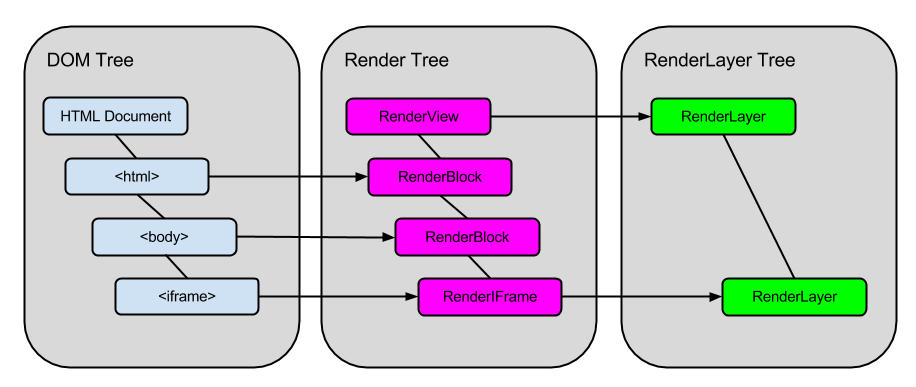
\includegraphics[scale=0.46]{rendering-trees}
    \caption{
        \label{fig:rendering-trees}
        Rendering Trees \cite{bib:chromium-oopifs}
    }
\end{figure}

\noindent
Az \ref{fig:rendering-trees} ábra szemlélteti, hogyan is állnak össze ezek a struktúrák.
A \texttt{DOM Tree} és a \texttt{Render Tree} szinte azonos, annyi különbséggel, hogy
a \texttt{Render Tree} csak a megjeleníthető \texttt{Node}-okat tartalmazza.
A \texttt{RenderLayer Tree} a \texttt{Render Tree} egy lecsupaszított változata, amit a
megjelenítő komponens (renderer) fog használni a rajzoláshoz.
A \texttt{RenderLayer}-ből elérhetőek a \texttt{RenderObject}-ek, a \texttt{RenderLayer Tree}
szerkezete pedig, hordozza azt az információt, hogy milyen sorrendben kell kirajzolni
\texttt{RenderObject}-eket és, hogy azok között milyen átfedések lehetnek.

Az, hogy a rajzolás hogyan történik az függ attól, hogy van e elérhető hardveres gyorsítás.
Ha nincs, akkor szoftveres renderelés történik. A szoftveres renderelés során a rajzoló
algoritmus bejárja a \texttt{RenderLayer Tree}-n keresztül a \texttt{RenderObject}-eket és
azokat egy közös bitmapre rajzoltatja ki. Ha kész, ez a bitmap lesz elküldve egy másik
processz (Browser Process) számára megjelenítésre. Szoftveres renderelés esetén a rajzolást
a Skia grafikus motor végzi.

Ha van elérhető hardveres gyorsítás, akkor az eljárás valamivel bonyolultabb. Ebben az
esetben, a \texttt{RenderObject} nem bitmapbe ``rajzolja bele magát'', hanem 3D API-n
keresztül (OpenGL vagy Windowson esetleg D3D) utasításokat küld közvetlenül a GPU
utasítás pufferébe (command buffer) végrehajtásra. Ezt az eljárást már a
Chrome Compositor (CC) végzi.
\cite{bib:chromium-gpu, bib:chromium-oopifs}

\subsection{Chrome Compositor (CC)}
A Chrome Compositor nem része a Blinknek (ahogy a Skia sem). Ennek az az oka,
hogy a Chromium a böngészőalkalmazás felhasználói felületének (GUI) összeállításához is
nyújt API-kat (pl. Aura). A Chromium a GUI megrajzolásához is a Chrome Compositort
használja.

Ahhoz, hogy a compositor ki tudja rajzolni a DOM-ban tárolt tartalmat, további layer
absztrakciókra van szükség:
\begin{center}
    \texttt{RenderLayers} $\rightarrow$ \texttt{GraphicsLayers} $\rightarrow$
    \texttt{WebLayers} $\rightarrow$ \texttt{CC Layers}
\end{center}
A compositor a végeredményt nem bitmapbe, hanem textúrába rajzolja. Az elkészült
textúrák a GPU memóriájában vannak tárolva és úgynevezett \textit{texture mailbox}
segítségével azonosítják őket.
A texture mailbox egy OpenGL kiterjesztés, ami egyedi és globális
string azonosítót rendel a textúrához és lehetővé teszi, hogy az más OpenGL contextben
is elérhető legyen.
\cite{bib:chromium-gpu, bib:chromium-oopifs}

A texture mailbox-nak hála az összeállított képet nem kell az IPC-n (Inter-Process
Communication) keresztül megosztani a processzek között (mint a szoftveres rendering
esetében), hanem a GPU memórián keresztül bármelyik processz hozzáférhet a textúrához.
Ezzel a megoldással elég csak a textúra azonosítót (mailbox) átküldeni IPC-n.
\cite{bib:chromium-texture-mailbox}

\subsection{Multi-processz Architektúra}
Chromium volt az egyik első olyan böngésző, ami úgy lett megtervezve, hogy több processzre
legyen felosztva. A WebKit multi-processz architektúrára épülő API-ja
-- a WebKit2\footnote{A QtWebKit Quick API-ja a WebKit2-re épül} --
is a Chromium megvalósításáról mintázta a multi-processz architektúráját.
\cite{bib:webkit-webkit2}

A multi-processz architektúrán alapuló böngésző alapgondolata az, hogy a böngészőalkalmazás
UI-ért felelős része saját processzben fut, míg a weboldalak megjelenítésért más
processzek felelnek. Ennek több előnye is van: \cite{bib:chromium-blog-multi-process}
\begin{description}
    \item[Felhasználói élmény]
        Előfordulhat, hogy egy weboldalon futó script (vagy ``webalkalmazás'')
        nagyon leterheli a böngészőt. Ha ez a script és a UI egy processzben fut,
        akkor ezek nagyobb valószínűséggel vonnak el egymástól erőforrást. Ha külön
        processzben, egymástól függetlenül futnak, kisebb valószínűséggel alakul ki
        köztük versenyhelyzet, így a UI nagyobb CPU használatnál is ``reszponzívabb''
        lehet.
    \item[Biztonság]
        Egyes processzek sandboxban futhatnak. Ezáltal nem férhetnek hozzá a rendszer
        olyan erőforrásaihoz, ami veszélyes lehet (pl. merevlemez, hálózat,
        videó memória, stb).
        Továbbá a különböző weboldalakat megjelenítő processzek egymástól is el vannak
        különítve, így egy ártalmas oldal, vagy plugin nem férhet hozzá más oldalon használt
        ``kényes'' információhoz (pl. jelszó).
    \item[Hibatűrés, Robosztusság]
        Ha egy oldal betöltésekor vagy egy bővítmény futtatásakor hiba történik és
        összeomlik, az nem rántja magával a teljes böngészőt. Hiba esetén a UI és más
        megnyitott oldalak, tabok megmaradnak.
\end{description}

A multi-processz architektúrának hátrányai is vannak: ez a megoldás sokkal
erőforrás-igényesebb, és a megvalósítás is bonyolultabb (több hibalehetőség).
A processzek használata memória többletköltséggel jár. A futtatható processzek
számát limitálni kell, mert túl sok processz jelentős lassulást okozhat (pl. az ütemező
többletköltsége miatt).

A processzek IPC-n (Chromium's IPC System) keresztül kommunikálnak egymással.
A Chromiumban 4 fő processz típust különböztetünk meg:

\subsubsection{Browser Process}
Ez az a processz, ahol maga böngésző alkalmazás (UI) fut. Ez felelős megjelenítésért,
a felhasználói események és a tabok kezeléséért. Ez a fő processz, ami a többi processzt
kezeli (indítja, leállítja, stb.) és csak egy van belőle. Hozzáfér a rendszer erőforrásaihoz,
viszont nem tölt be vagy dolgoz fel web tartalmat.

\subsubsection{Render Process}
A renderelő motor egy nagyon összetett és bonyolult szoftver komponens. Szinte lehetetlen
olyat implementálni, ami sosem hibázik és/vagy omlik össze. \cite{bib:chromium-multi-process}
Ezért érdemes az egymástól független oldalak renderelését egymástól független
processzekben végrehajtani. Amennyiben egy Render Process összeomlik, arról a
Browser Process értesül és az oldal helyett az \ref{fig:sad-tab} ábrán látható,
úgynevezett, ``sad tab'' értesítést jeleníti meg.

\begin{figure}[h]
    \centering
    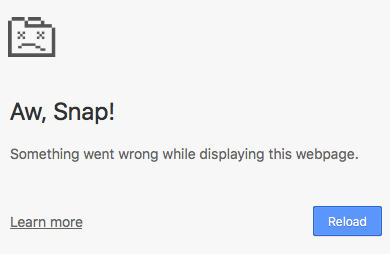
\includegraphics[scale=0.8]{sad-tab}
    \caption{
        \label{fig:sad-tab}
        Sad Tab
    }
\end{figure}

Mivel a Chromiumban a renderelésért a Blink felel, ezért az is a Render Processben fut.
A Blink az, ami közvetlenül feldolgozza a webes tartalmat, ezért jellemzően a
Render Processt sandboxban futtatják, így a potenciálisan kártékony webes kódok nem
férhetnek hozzá a rendszer erőforrásaihoz vagy más betöltött webes tartalomhoz.

A Chromiumban különböző parancssori kapcsolókkal is beállítható processz modellek
vannak definiálva:
\begin{description}
    \item[Process-per-site-instance]
        Minden \textit{site}\footnote{Site alatt olyan weboldalak csoportját értjük, amelyek
        közös beregisztrált domain néven osztoznak} külön processz.
        Ha ugyanaz a site kétszer van megnyitva, akkor az is két külön processz lesz.
    \item[Process-per-site]
        Különböző site-ok külön processzbe kerülnek. Az előzővel ellentétben, ha egy site
        kétszer van megnyitva, akkor azok közös processzbe kerülnek.
    \item[Process-per-tab]
        Minden tab külön processz. Több tab kerülhet közös processzbe, ha függnek egymástól.
    \item[Single Process]
        A ``hagyományos'', egy-processzes modell. Nincs külön Render Process. A rendering
        a Browser Processben, külön szálon (thread) történik.
\end{description}

\noindent
Alapértelmezetten a \textit{Process-per-site-instance} modellt használja a Chromium.
Ettől függetlenül azonban előfordulhat, hogy több site is osztozik, ugyanazon a processzen.
Erre vagy akkor van szükség amikor két site hivatkozik scriptből egymásra (függnek
egymástól), vagy amikor a futó Render Processek száma elér egy korlátot.
\cite{bib:chromium-process-models}

\subsubsection{Plugin Process}
A pluginok okozzák a legtöbb problémát egy böngésző stabilitásának szempontjából. A plugint
egy harmadik fél készíti, ezért a Chromiumnak nincs befolyása afelett, hogy milyen
erőforrásokat használ. Biztonsági és stabilitási megfontolásból érdemes a pluginokat nem
a Browser Processben futtatni. A legtöbb plugin azonban nem futhat sandbox környezetben,
mivel olyan képességekkel bővítik a böngészőt, amelyekhez szükség van hozzáférésre a rendszer
erőforrásaihoz. Ezen megszorítás miatt a Render Process nem jöhet számításba, így új
processz típusra van szükség, ami a Plugin Process.
\cite{bib:chromium-plugins}

\subsubsection{GPU Process}
A renderelés a Render Processben történik, viszont ez a processz sandboxban fut és ezért
nem küldhet parancsokat GPU-nak. Hardveres gyorsítás esetén a compositingot és a rajzolást
egy külön, nem sandbox környezetben futó processzben\footnote{A Chromium úgy is
konfigurálható, hogy a GPU Process feladatát a Browser Process lássa el} kell elvégezni.
Erre a célra szánt processz típus a GPU Process.
\cite{bib:chromium-gpu}

\subsection{Chromium Content Module}
A Content Module a Chromium az a része, ami megvalósítja az előző fejezetben bemutatott
multi-processz architektúrát. Itt van még megvalósítva az összes támogatott
web platform funkcionalitás (például: HTML5, WebRTC, WebGL, stb.), illetve
a hardveres GPU gyorsítás is. Böngészőalkalmazás specifikus funkcionalitások, nem részei
Content Module-nak. Lényegében csak olyan funkciókat implementál ami a web tartalom
megjelenítéséhez\footnote{\textit{content} = web tartalom} szükséges.
Ezekre a legtöbb böngészőt integráló alkalmazásnak szüksége van.
\cite{bib:chromium-content-module}

Az opcionális böngésző funkcionalitásokat a beágyazó
alkalmazásnak\footnote{A Chromium Content Module-t beágyazó alkalmazás például a Chrome}
kell implementálnia, viszont egyes funkciók szorosan kötődhetnek a Content Module-hoz,
így szükség van egy interfészre is, amin keresztül a funkciók megvalósíthatóak és
testreszabhatóak a beágyazó alkalmazásban anélkül, hogy a Chromium forráskódját módosítani
kellene. Ez az interfész a Chromium Content API.

\subsubsection{Chromium Content API}
A Content API megtervezésekor a WebKit API-t vették alapul, hogy a WebKit fejlesztők
könnyebben áttérhessenek. A Content API \textit{unstable}, ami azt jelenti, hogy az minden
új kiadásban változhat, ezért az azt használó alkalmazást is minden Chromium frissítés után
nagy valószínűséggel változtatni kell.

A Content Module a beágyazó alkalmazást interfészeken (Delegate, Observer)
és callback függvényeken keresztül értesíti az eseményekről, változásokról (például,
hol tart a web oldal letöltése vagy sikeres volt-e a letöltés) vagy éppen
kér le adatokat (például, kell-e megjeleníteni hiba üzenetet, ha nem sikerül letölteni egy
oldalt). Az ilyen interfészek metódusainak törzse üres a Content Module-ban, ezeket a
beágyazó alkalmazásnak kell megvalósítania és a Content Module hívja meg őket szükség esetén.

Ezeken kívül vannak olyan interfészek is, amelyeket a Content Module implementál
(például, oldal betöltése: \texttt{LoadURLWithParams()} vagy az URL lekérdezése:
\texttt{GetVisibleURL()}).
Ezek \textit{pure abstract} interfészek, mivel csak egy megvalósításuk lehet
és az is a Content Module-on belül. \cite{bib:chromium-content-api}

\subsubsection{Chromium Content Shell}
\begin{figure}[h]
    \centering
    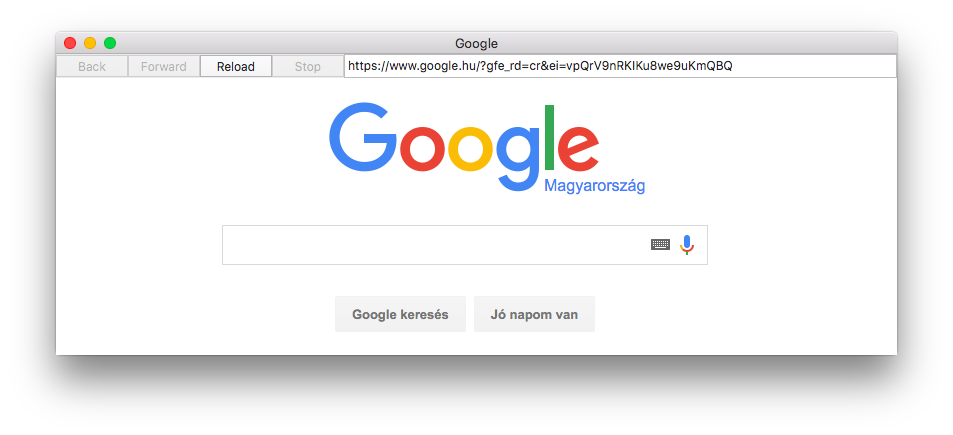
\includegraphics[scale=0.40]{content-shell}
    \caption{
        \label{fig:content-shell}
        Content Shell
    }
\end{figure}
Az \ref{fig:content-shell} ábrán látható alkalmazás a Content Shell. Ez a lehető
legegyszerűbb böngészőalkalmazás, ami a Content API-ra épül. Arra használják, hogy a
Content Module-t és a Blinket tesztelhessék, debuggolhassák anélkül, hogy egy teljes
böngészőalkalmazást (pl. Chrome) le kellene fordítani.

\subsection{Felépítés}
Az eddigiek alapján a Chromiumot 3 rétegre oszthatjuk fel:
\begin{description}
    \item[Chrome]
        Felhasználói felület (UI) és böngészőalkalmazás funkciók
        (pl.: böngészési előzmények, könyvjelzők, favicon, stb.)
    \item[Blink]
        Webes tartalom feldolgozása és renderelése. A V8 JavaScript motor a
        Blinken keresztül érhető el és közös processzben futnak.
    \item[Content]
        Ez a réteg valósítja meg a multi-processz architektúrát,
        felel a web platform funkciókért és a hardveres GPU gyorsításért.
\end{description}
A \ref{fig:chromium-architecture} ábra mutatja, hogyan is állnak össze a Chromium rétegei.
A Blink böngészőmotor ``WebKit'' elnevezéssel van jelölve.
A legfelső réteg a Chrome, helyére a saját beágyazó alkalmazás kerül.

\begin{figure}[ht]
    \centering
    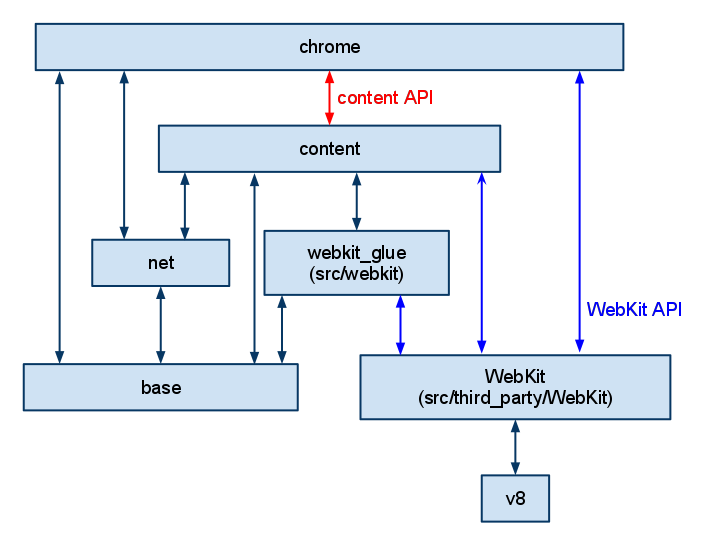
\includegraphics[scale=0.6]{chromium-architecture}
    \caption{
        \label{fig:chromium-architecture}
        Chromium Architecture \cite{bib:chromium-content-module}
    }
\end{figure}


\subsection{Release}
Egy Chromium release verzió száma 4 részből tevődik össze:
\begin{verbatim}
    MAJOR.MINOR.BUILD.PATCH
\end{verbatim}
A dolgozatomban a főverzió számra (\texttt{MAJOR}) hivatkozok.
A Chromium közösség előre tervezett menetrend szerint 1-1.5 havonta vált főverzió számot
(ad ki új release-t).
Dolgozatom készítése idején az 51-es verziójú volt a legfrissebb stabil kiadás.
Az itt leírtak erre a verzióra vonatkoznak.


\section{Qt}
A Qt egy nyílt forrású, cross-platform alkalmazás keretrendszer. Úgy ahogy a Chromium, úgy a
Qt is elérhető napjaink legnépszerűbb desktop és mobil operációs rendszerein. Ez a
keretrendszer nyújt C++ függvénykönyvtárakat (library), bindingokat más programozási
nyelvekhez (pl.: Python, Java), saját deklaratív programozási nyelvet (QML), saját integrált
fejlesztői környezetet (QtCreator), saját build rendszert (qmake) és kiterjesztéseket is a
C++ programozási nyelvhez (pl.: signal--slot modell).
\cite{bib:qt-wiki-about-qt}

\subsection{Történeti áttekintés}
\subsubsection{1995-2000}
A Qt első verzióját 1995-ben adta ki a Trolltech. Akkor még a projekt egy cross-platform GUI
fejlesztői keretrendszernek indult. Pár évvel később (1998-ban), jelent meg a
KDE (K Desktop Environment) első verziója, amely Qt-re épült. A KDE egyhamar az egyik
legnépszerűbb Linuxos asztali környezetté nőtte ki magát és talán ennek tudható be a Qt
mai napig tartó népszerűsége is. A Qt eszköztára az évek során fokozatosan bővült.
Új API-k jelentek meg adatbázis kezeléshez (SQL), hálózati programozáshoz, multimédiás
alkalmazások készítéséhez, XML dokumentumok feldolgozásához stb.

\subsubsection{2000-2008}
2000-ben jelent meg a Qt-ra épülő Qt/Embedded keretrendszer Linuxos beágyazott eszközökre.
Ezzel az új technológiával a Qt meg is jelent az első okos telefonokon (2003: Motorola A760)
és a korabeli PDA-kon. 2006-ban a Trolltech kiadta saját fejlesztésű mobil telefonját
Greenphone néven.

\subsubsection{2008-2011}
Talán a Trolltech beágyazott platformokon és mobil telefonokon szerzett tapasztalata
miatt került arra sor, hogy 2008-ban, az akkori egyik vezető mobiltelefon gyártó -- a Nokia --
felvásárolta a céget. A következő pár évben a fejlesztés még inkább a mobil eszközök
felé tolódott el. Ezekben az években azokon a területeken, amelyek nem voltak érintettek a
mobil platformok által, jóformán nem is történt fejlesztés.
2010-ben kiadott 4.7-es verzióban két nagyon fontos újítás (teljesen új komponens) jelent meg:
a QtWebKit és a QtDeclarative.

A WebKit az Apple által fejlesztett nyílt forrású böngészőmotor. A Qt erre építette saját
böngészőmotorját, a QtWebKitet. A QtWebKit a WebKittel szemben Qt-s API-val rendelkezik és az
alacsony szintű műveleteket is -- mint a hálózatkezelés vagy a tartalom kirajzolása -- a Qt
végzi. A WebKit 2 régi KDE-s projektekre épül: KHTML-re (WebCore) és a
KJS-re (JavaScriptCore). A sors iróniája, hogy amikor 2001-ben az Apple fejlesztői forkolták
ezeket a projekteket a céljuk éppen az volt, hogy egy a Qt-tól független új böngészőmotort
alkossanak.

Az új verzió másik fontos újítása a Qt Quick keretrendszer és a QML nyelv (QtDeclarative)
megjelenése volt. A QML egy új deklaratív programozási nyelv, a Qt Quick pedig egy
eszközkészletet nyújtott hozzá. Ezek segítségével a Qt új lehetőségeket nyitott grafikus
felhasználói felületek megvalósítására. Ez az új technológia a mobil fejlesztés szempontjából
jelentős előrelépés volt. A legnagyobb előnye (a könnyű használhatóságot és a gyors
fejlesztési ciklust nem számítva), hogy mobil alkalmazás felhasználói felületének
lefejlesztéséhez nincs szükség szimulátorra, hiszen a QML-ben írt alkalmazás
platform független és ugyanúgy fut/néz ki desktopon mint mobilon.

\subsubsection{2011-2013}
2011 elején a Nokia szerződést kötött a Microsofttal. A Nokia készülékek elsődleges
platformja a Windows Phone lett, így a Nokia elkezdte fokozatosan leépíteni a
szoftver kutatás-fejlesztés részlegét. 2012-re a Qt teljes egészében a Digia
tulajdonába került.

A 2012-es év pozitív változást is hozott, az év végén megjelent a Qt 5.0-ás verziója.
Az új verzió API-ja nem sokban tér a 4-estől, így az új API szinte teljesen kompatibilis
maradt a régivel. Az igazán fontos változás a Qt kód struktúrájában történt.
A 4-es verzióban a kódot már modulokra bontották, hogy a Qt-s alkalmazások méretét
csökkentsék azzal, hogy a nem használt modulokat (gyakorlatilag függvénykönyvtárakat) nem
linkelik az alkalmazáshoz.
Az 5-ös verzióban a fejlesztők tovább mentek: a keretrendszert több,
kisebb modulra bontották és az összetartozó modulokat közös repositoryba helyezték
(komponensek vagy alprojektek). Ezzel megszűnt a 4-es verzió ``egy-repositorys'' modellje
és így a modulok/komponensek egymástól függetlenül is kiadhatóvá, verziózhatóvá váltak.
Az új projektek/modulok saját repositoryait a \texttt{qt5} top-level repository gyűjti össze,
amely hivatkozásokat (git submodule) tartalmaz a alprojektek repositoryjaira.

Az 5-ös verzió másik újítása Qt Quick2 modul volt. A Qt Quick első verziója (Qt Quick1) a
\texttt{QGraphicsView}-ra épül, ami szoftveres renderelést használ a megjelenítéshez.
Ez a megoldás lassú, ráadásul widget függőséggel is jár (Qt Widgets modul).
A Qt Quick2 API-ja kompatibilis maradt a Qt Quick1-el, viszont teljesen újraírták.
Megszűnt a widget függőség mivel ezentúl a Qt Quick2 saját Qt Quick Scene Graph-ot valósít
meg. Ez a scene graph Open GL ES 2.0-ra vagy Open GL 2.0-ra épül, így a renderelés a GPU-n
történik. Ez a megoldás sokkal gyorsabb, viszont nem támogatott olyan platformokon, ahol
nem elérhető az Open GL 2 vagy újabb verziója.

2013-ban a Qt fejlesztői úgy döntenek szakítanak a WebKittel és, hogy böngésző motor
API-jukat ezentúl a Chromium felé építik. \cite{bib:qt-blog-introducing-qtwebengine}
Az új komponenst Qt WebEngine-nek hívják és 5.4-es verzióban jelent meg először.
\cite{bib:qt-wiki-qt-history}

\subsubsection{2014-napjainkig}
2014-ben a Qt részlege kivált a Digia-ból és létrejött a \textit{The Qt Company},
mint a Digia leányvállalata. A kiválás oka, hogy a Qt üzleti logikája és piaca eltér a
Digia-étól, ezért másfajta vezetésre, fejlesztésre és befektetési tervre van szükség.
Ez a folyamat még 2016-ban is tart és terv szerint 2016 májusában a The Qt Company megjelenik
a tőzsdén is.
\cite{bib:qt-about-us}

A Qt hányattatásai ellenére még ma is töretlen népszerűségnek örvend és talán az egyik
legjobb elérhető C++ alkalmazás keretrendszer a piacon. Ezt bizonyítja,
hogy több, napjainkban is népszerű és széles körben elterjedt alkalmazás is a
Qt keretrendszerre épít. Mint például Skype, Google Earth, VirtualBox,
a VLC média lejátszó és a Spotify is.

\subsection{Modulok és Komponensek}
A 4-es Qt verzióban megtörtént az első lépés a modularizáció felé: minden modul külön
függvénykönyvtárként jelenik meg, a korábbi egyetlen Qt függvénykönyvtár helyett.
Ennek előnye, hogy a fejlesztőnek nem kell olyan modulokat az alkalmazásához linkelnie,
amit nem is használ.

\begin{figure}[h]
    \centering
    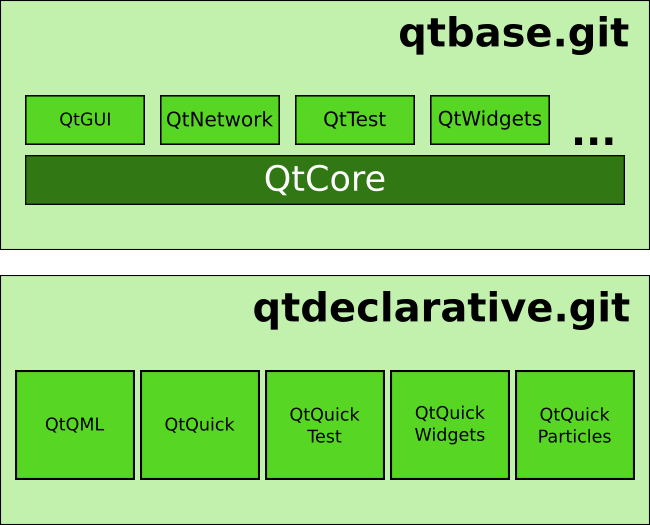
\includegraphics[scale=.66]{qt-repos-and-modules}
    \caption{
        \label{fig:qt-repos-and-modules}
        Qt repository-k és modulok
    }
\end{figure}

Az 5-ös Qt verzióban kiterjesztették a modularizációt a projekt struktúrájára is. A projekt
többé nem egy nagy közös repository, hanem több önálló repositoryból áll össze, melyeket
a modulok szerint választottak szét. Ennek a modellnek több előnye is van: a moduloknak
saját verzió számuk lehet, ezért a Qt release-től függetlenül is kiadhatóak. Fejlesztés
szempontjából a buildelés és tesztelés rugalmasabb és gyorsabb lett, hiszen változás esetén
csak a modult és annak függőségeit kell újra buildelni.

Qt 5-ben a modulokat két kategóriába sorolják: \textbf{Qt Essentials} és
\textbf{Qt Add-Ons} \cite{bib:qt-doc-qtmodules}.
Az Essential modulok nyújtják a Qt alap funkcionalitását, amit a legtöbb Qt-s alkalmazás
használ. Ezeknek a moduloknak működniük kell az összes támogatott platformon, az 5-ös
főverzión belül a bináris és az API kompatibilitás garantált.

Az Add-on modulok nem általános célú, opcionális modulok. Nem garantált, hogy minden
támogatott platformon működnek és az egyes verziók sem biztos, hogy kompatibilisak egymással.
A kifutó Qt modulok (pl.: Qt Script) is a az Add-ons kategóriába kerülnek addig, amíg
véglegesen el nem távolítják őket. A QtWebEngine moduljai is Add-onok, mivel nem általános
célúak, a legtöbb alkalmazásnak nincs szüksége böngésző funkciókra.

Ha egy Qt-s alkalmazás használ egy Qt modult, akkor azt annak a projekt fájljában meg kell
adni:
\begin{lstlisting}[title=app.pro]
 QT += network widgets qml quick
\end{lstlisting}
Ez alól kivétel a Qt Core és a Qt GUI modul. A Qt Core modult
minden Qt-s alkalmazás használja, ezért azt a Qt build rendszere implicit linkeli.
Ebben a modulban vannak megvalósítva a Qt típusok és adatszerkezetek, a Qt specifikus nyelvi
elemek és makrók (pl.: \texttt{Q\_OBJECT}, \texttt{signals}, \texttt{slots}),
smart pointerek, stb. A Qt GUI\footnote{A Qt GUI modulról bővebben a \ref{sec:qt-gui}
fejezetben lesz szó.} modulra a grafikus felhasználói felület megvalósításához van szükség.
A Core modulhoz hasonlóan implicit linkelődik az alkalmazáshoz viszont ez már letiltható, ha
a következő sort adjuk a projekt fájlhoz:
\begin{lstlisting}[title=app.pro]
 QT -= gui
\end{lstlisting}

Ahogy a Qt-s alkalmazások, használnak egy Qt-s modult, úgy a Qt-s modulok is függhetnek
egymástól. Az alkalmazáséhoz hasonlóan, a modul projekt fájljában is jelölni kell a
függőséget. Továbbá ez a függőség komponensek közötti függőséget is jelent, hogy ha
a hivatkozott modul egy másik repository-ban van. A komponens függőségeit a
\texttt{sync.profile} scriptben kell felsorolni:
\begin{lstlisting}[title=sync.profile]
 %dependencies = (
    "qtbase" => "",
    "qtdeclarative" => "",
    "qtxmlpatterns" => "",
    "qtquickcontrols" => "",
    "qtwebchannel" => "",
 );
\end{lstlisting}
Habár a QtBase komponens minden más komponens függősége, azt explicit meg kell adni.
Az \ref{fig:qtwebengine-dependencies} ábra mutatja, hogy a fenti \texttt{sync.profile} script
alapján a QtWebEngine függőségei hogyan alakulnak.

\begin{figure}[ht]
    \centering
    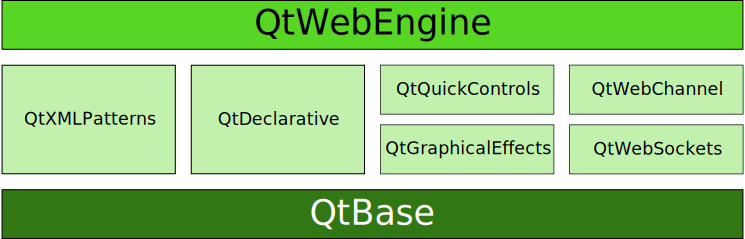
\includegraphics[scale=.6]{qtwebengine-dependencies}
    \caption{
        \label{fig:qtwebengine-dependencies}
        QtWebEngine függőségei
    }
\end{figure}

\subsection{GUI}
\label{sec:qt-gui}
A Qt keretrendszer grafikus felhasználói felületek (GUI) megvalósítására gazdag
eszközkészletet kínál a fejlesztők számára. A Qt GUI modul \cite{bib:qt-doc-qt-gui} az,
amely alacsony szintű API-t nyújt 2D (rasztergrafika) és 3D (OpenGL API) rajzoláshoz,
esemény kezeléshez, képek és szövegek megjelenítéséhez.
Egy grafikus felület megvalósításához nem érdemes közvetlenül a Qt GUI modul
alacsony színtű API-ját használni. A Qt nyújt magasabb szintű, Qt GUI-ra épülő API-kat is
\cite{bib:qt-doc-user-interfaces}.
Jelenleg két egymástól eltérő megoldás is elérhető: \textbf{Widget} és a \textbf{Quick}.

\subsubsection{Widget}
A widget API-n \cite{bib:qt-doc-qt-widgets} keresztül ``hagyományos'' felhasználói
felületeket lehet megvalósítani, melyeknek megjelenítéséhez a Qt a futtató operációs
rendszer stílusát adja (\textit{native look'n'feel}). A widgetek olyan statikus GUI elemek,
amelyekből desktop alkalmazások grafikus felülete felépül. Információt jelenítenek meg és
felhasználói eseményekre reagálhatnak. Ilyen Qt widget elemek például:
gomb (\texttt{QButton}), címke (\texttt{QLabel}), görgetősáv (\texttt{QScrollBar}), stb.
Az a widget, aminek nincs szülője, az az ablak (\texttt{QWindow})

A Qt beépített widgetjei a \textbf{Qt Widgets} modulból elérhetőek, de saját widgetek is
készíthetőek. A widgeteket és azok tartalmát a \texttt{QGraphicsView} jeleníti meg. A rajzolás
szoftveresen történik, nincs hardveres gyorsítás.

A Qt Widgets modul a widgeteken kívül tartalmaz API-t a widgetek megjelenítésének
testreszabására (\texttt{QStyle}) és beépített stílusokat is natív megjelenéshez különböző
platformokon. A widgetek elrendezésére a modul \texttt{QLayout} osztályai használhatóak.

A widget alapú GUI-t első sorban C++ API-n keresztül lehet felépíteni, de a Qt
keretrendszer tartalmaz egy Qt Designer elnevezésű alkalmazást is, aminek segítségével,
akár programozási ismeret nélkül össze lehet állítani a egy felhasználói felületet.
A Qt Designer a widgeteket fastruktúrába rendezi és XML formátumban tárolja egy \texttt{.ui}
kiterjesztésű fájlban. Az XML fájlból a User Interface Compiler (uic) generál buildelhető
C++ forrás állományt.

\subsubsection{Quick}
Az új Quick technológia segítségével modern megjelenésű, dinamikus elemekből felépített,
``fluid'' GUI-t lehet összeállítani. Megvalósítás ``deklaratív módszerrel'' történik, ami
magasabb szintű, mint a widget API esetében használatos imperatív paradigma: nem azt kell
leprogramozni, hogyan legyen megjelenítve a GUI, hanem azt, hogy hogyan nézzen ki
(mint például a HTML esetében). A technológia használatához alapvetően 2 modulra van
szükség: \textbf{Qt QML}-re és a \textbf{Qt Quick}-re\footnote{Mindkét modul a QtDeclarative
projekt része}.

A Qt egy saját nyelvet nyújt a deklaratív programozáshoz és ez a QML (Qt Modeling Language)
\cite{bib:qt-doc-qt-qml}. A QML nyelv a Qt QML modulon keresztül válik elérhetővé. A modul
rendelkezik C++ és QML API-val is, hogy a QML nyelv saját típusokkal és funkciókkal bővíthető
legyen. A Quick GUI akár ezen a C++ API-n keresztül is megvalósítható, de erre a célra
sokkal inkább a QML nyelv használata ajánlott.

A QML nyelv ``JSON-szerű'' szintaxissal írja le a UI komponensek hierarchiáját és
kapcsolatait. A QML programot egy külön erre a célra fejlesztett JavaScript motor dolgozza
fel és hajtja végre, ez a v4. Ezáltal lehetővé válik, hogy a UI kódja akár futásidőben is
§dinamikusan változtatható legyen. JavaScript kód szabadon hozzáadható a QML forráshoz, így
akár logikát is meg lehet valósítani a QML programon belül. JavaScript kód használatánál
érdemes csak az eseménykezelésre szorítkozni és a többi vezérlést a Qt QML modul C++ API-ján
keresztül C++ nyelven megvalósítani.

Habár a Qt QML modul rendelkezésünkre bocsájtja a QML deklaratív nyelvet, az még
nem rendelkezik olyan elemekkel, amelyekből össze lehetne állítani egy grafikus felületet.
Előre gyártott GUI elemeket a \textbf{Qt Quick} és a \textbf{Qt QuickControls} modulok
szolgálgatják \cite{bib:qt-doc-qt-quick}. Ezekben majdnem minden elem megtalálható, mint ami
widget API-ban, sőt még több is. További lehetőség nyílik a felület elemeinek animálására
Qt Quick API-ján keresztül. A Qt Quick C++ API-ját használva pedig saját
\texttt{QQuickItem}-ek hozhatóak létre, melyek a Qt QML C++ API-ján keresztül QML típusként
regisztrálhatóak be a QML nyelvbe.

A Qt Quick modul felel a Quick GUI elemek megjelenítéséért és kirajzolásáért is.
Korábban (Qt Quick1) a rajzolás ugyanúgy történt, mint a widget esetén: az elemek a
\texttt{QGraphicsView}-ra voltak kirajzolva. Ez a megoldás lassú, különösen, ha egy folyton
változó dinamikus felhasználói felületről beszélünk. A jelenleg is használt Qt Quick verzióban
(Qt Quick2) jelent meg a Qt Quick Scene Graph \cite{bib:qt-doc-qt-quick-scene-graph}.
A Qt Quick Scene Graph a Qt Quick modul része, ezért nem használható önállóan, viszont van
publikus API-ja. A scene graph a UI elemeiből épített fa struktúra, amelyet aztán a modul
OpenGL ES 2.0 vagy OpenGL 2.0 API-n keresztül megjelenít. Emiatt a Quick technológia nem
használható olyan platformokon, ahol nem érhető el legalább az OpenGL 2.0 API.

\subsection{Web}
A Qt keretrendszerben nem a QtWebEngine az egyetlen komponens/modul ami a
webhez, web alkalmazásokhoz nyújt API-t.

\subsubsection{QtWebKit}
A QtWebKit a nyílt forrású WebKit böngésző motor portja. A WebKit API felé két fajta Qt-s
API-t implementál: C++ API-t a Widget alkalmazásokba való beágyazáshoz és QML/Quick API-t a
Quick alkalmazásokhoz. A C++ API szinkron, mivel a single-process architektúrájú WebKit
API-ra (WebKit1) épül. Ezzel szemben a Quick integrációt lehetővé tevő QML API aszinkron,
mert az már a multi-process WebKit2-re épül.

A QtWebKit a Qt 4.7-es verziójában jelent meg. A Chromium--WebKit szétválás után a
fejlesztése leállt és csak karbantartási munkálatokat végeztek rajta. A Qt 5.5-ös kiadásban
már elavultnak (deprecated) számít az 5.6-os verzióból már a bináris csomagokat is
eltávolították, csak QtWebKit forráskódja érhető el. A QtWebKit leváltására a Chromiumra
épülő QtWebEngine-t hozták be.

\subsubsection{QtWebView}
A QtWebKit sosem volt támogatott mobil platformokon (Embedded Linuxon igen) és ez jelenleg
hivatalosan igaz a QtWebEngine-re is. Azonban, a mobil platformok (pl. Android, iOS, WinRT)
biztosítanak natív API-t (WebView) a webes tartalmak megjelenítésére. Biztonsági
megfontolásból más módon a mobil alkalmazások nem is férhetnének hozzá web tartalomhoz.

A QtWebView komponens/modul \cite{bib:qt-doc-qt-webview} ezeket a natív API-kat fedi el
(wrapper) és implementál felettük egységes, Qt API-t. Amennyiben nincs elérhető (vagy
támogatott) web API a platformon, akkor a QtWebEngine-t próbálja használni (fallback).
A QtWebView-nak csak QML/Quick API-ja van.

\subsubsection{QtWebSockets}
A WebSocket egy olyan protokoll, amely kétirányú kommunikációt biztosít a web felett.
A kommunikáció kliens és szerver között történik. A legtöbb modern böngésző integrálja a
WebSocket klienst. A QtWebSockets \cite{bib:qt-doc-qt-websockets} C++ és QML/Quick API-t
biztosít mind WebSocket kliens és szerver megvalósításához.

\subsubsection{QtWebChannel}
A QtWebChannel komponens/modul \cite{bib:qt-doc-qt-webchannel} a Qt 5.4-es verziójában jelent
meg. Olyan alkalmazások esetében, amelyek beépített HTML tartalmat jelenítenek meg szükség
lehet olyan megoldásra, amelynek segítségével a WebView-ban futó webalkalmazás
(JavaScript/HTML) és a natív alkalmazás (QML/C++) kommunikálni tud
\cite{bib:kdab-qt-webchannel}.

A single-process QtWebKit widget API esetén ennek megvalósítása nem jelentett különösebb
problémát, viszont egy multi-process architektúrára épülő motor (WebKit2 vagy Chromium)
a megvalósítás már sokkal bonyolultabb. Erre a problémára nyújt megoldást a QtWebChannel.

A QtWebChannel segítségével egy \textit{Qt MetaObject}-et (\texttt{QObject}) lehet
``meghirdetni'' szerver oldalon, a kliens oldal pedig ezt a MetaObject-et tudja használni.
A komponens szerver oldalra nyújt QML és C++, a kliens oldalra pedig JavaScript API-t.
A kliens oldalon megjelenő JavaScript objektum a szerver oldali Qt MetaObject másolata. A két
objektum szinkronizálva van, a property változtatások és a Qt-s szignálok mindkét oldalon
megjelennek.

Ez úgy valósul meg, hogy a QtWebChannel szerializálja Qt MetaObject-et majd átküldi
a kliensnek. A kliens oldali API a szerializált Qt MetaObject-ből JavaScript
object-et gyárt, amely képes kommunikálni az eredeti object-el. A kommunikáció történhet
QtWebSockets segítségével, de akár IPC-n keresztül is.

\subsection{Release}
Egy Qt release verzió száma 3 részből tevődik össze:
\begin{verbatim}
    MAJOR.MINOR.PATCH
\end{verbatim}
A dolgozatomban bemutatott fejlesztések mind az 5-ös főverzióban (\texttt{MAJOR})
jelentek meg. Ahol ez egyértelmű feltüntetem az alverzió számot is (\texttt{MINOR}).
A Qt közösség előre tervezett menetrend szerint fél évente vált alverzió számot (ad ki új
release-t). Dolgozatom készítése idején a Qt 5.6 a legfrissebb stabil kiadás, viszont egyes
bemutatott funkcionalitások, majd csak a Qt 5.7-ben lesznek elérhetőek.

\section{QtWebEngine}
A QtWebEngine \cite{bib:qt-doc-qtwebengine-overview} váltotta le a QtWebKitet a Qt
keretrendszer 5.4-es verziójában. A célja megegyezik a QtWebKitével: webes tartalom
integrálása és manipulálása Qt alkalmazásban. A QtWebEngine a Chromiumra épül, pontosabban a
Chromium Content Module unstable API-ja -- Chromium Content API -- felé implementál egy
stable API-t. Az \ref{fig:chromium-architecture} ábra alapján, a Chrome böngésző alkalmazás
helyére a Chromium \textit{stack} tetejére a QtWebEngine kerül és az lesz a Chromium Content
Module-t beágyazó ``alkalmazás''\footnote{QtWebEngine esetén inkább ``beépítő''
függvénykönvytárról van szó, mintsem alkalmazásról}.

A QtWebEngine fejlesztői forkolták a Chromiumot és ennek a forknak a karbantartása jelentős
mennyiségű munkát jelent a fejlesztőknek. Körülbelül 6 hetente jelenik meg új Chromium
verzió aminek változik az API-ja. Minden új verzió tartalmazhat biztonsági javításokat is,
amelyeket a Chromium fejlesztői nem backportolnak korábbi verziókba\footnote{A Chromiumnak
nincs LTS (Long Term Support) verziója}, ezért a rendszeres frissítésekre szükség van.
A biztonsági javítások, amikor ez megoldható \textit{cherry-pickelve} vannak a QtWebEngine
Chromium forkjába.

A QtWebEngine legnagyobb részét a Chromium fork forráskódja teszi ki, habár sok
nem használt Chromium komponens eltávolításra került (például a Chrome böngésző alkalmazás).
Viszont egyes ``backend'' komponensek, amelyek lecserélhetőek voltak QtWebKitben Qt modulokra,
már nem cserélhetőek le a Chromiumban. Ilyen például a Chromium \textit{network library}.

A web elemek kirajzolását viszont a Qt végzi. A mailbox texture azonosítók segítségével a
QtWebEngine hozzáfér a Chrome Compositor által összeállított textúrákhoz, amelyek a
megosztott OpenGL contexten vannak tárolva.
A textúrákból a QtWebEngine épít scene graph fát (\texttt{QSGNode} tree), amit majd a
Qt Quick Scene Graph rajzol ki. Emiatt, a Chromiumban a GPU process ki van kapcsolva,
mert a GPU-t a Qt használja, ami a Browser process-ben fut (\texttt{switches:kInProcessGPU}).

A scene graph függőség miatt a QtWebEngine nem működik olyan környezetben, ahol nincs
OpenGL ES 2.0 vagy OpenGL 2.0. Ez igaz a QtWebEngine widget API-jára is, mivel a web tartalom
kirajzolásának megvalósítása közös, így a Qt WebEngine Widgets modul sem működik Qt Quick
nélkül.

A QtWebEngine tartalmazza a QtWebEngine Processt és 3 modult: a Qt WebEngine és a
Qt WebEngine Widgets rendre a Quick és Widget API-kat valósítják meg. A Qt WebEngine Core
modul tartalmazza a Chromium forkot és QtWebEngine funkcionalitások közös megvalósítását,
amin a Quick és a Widget API-k osztoznak. A QtWebEngine felépítését a
\ref{fig:qtwebengine-architecture} ábra mutatja.

\begin{figure}[ht]
    \centering
    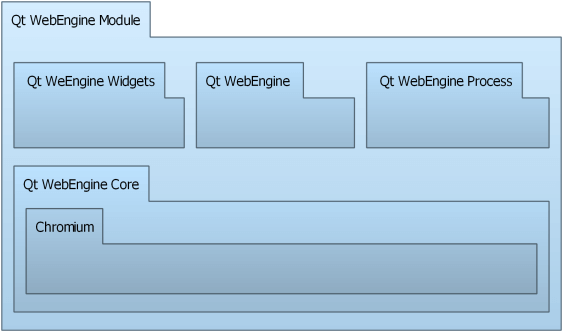
\includegraphics[scale=0.75]{qtwebengine-architecture}
    \caption{
        \label{fig:qtwebengine-architecture}
        QtWebEngine Architecture \cite{bib:qt-doc-webengine-overview}
    }
\end{figure}

\subsection{Process}
A QtWebEngine Process \cite{bib:qt-doc-qt-webengine-process} a Chromium Render Processt
bővíti ki és csomagolja magába. Különálló program saját belépési ponttal (\texttt{main()}
függvénnyel), amit a Browser Process indít el. Önálló fordítási egység, de a hozzátartozó kód
a QtWebEngine Core modulban található. Ez a processz felel a web tartalom megjelenítésért
(Blink) és a JavaScript kódok végrehajtásáért (V8). A processz OS X-en és Linuxon sandboxban
fut, Windowson a sandbox környezet még (Qt 5.7) nem támogatott.

\subsection{Core}
A Qt WebEngine Core modul \cite{bib:qt-doc-qt-webengine-core} tartalmazza a Chromium forkot
és implementálja a Chromium Content API interfészeit. Belső (\textit{internal}) API-ja elfedi
a publikus API-k (Widget, Quick) elől a Chromium Content API-t, így a publikus API-knak
nincsenek közvetlen Chromium függőségeik. A publikus API-k számára közös adapter interfészt
(\texttt{WebContentsAdapterClient}) definiál, amit a publikus API-nak kell megvalósítania.

A modul része a Qt Quick Scene Graph integráció is: ő hozza létre a Chromiumból
kinyert textúrákból a scene graph node-okat (\texttt{QSGNode}) és épít belőle fát a
megjelenítésre (compositing). Továbbá itt van megvalósítva a Browser Process és a Qt WebEngine
Process inicializációja (\texttt{WebEngineContext}), a QtWebEngine beállításainak továbbítása
a Chromium felé (\texttt{WebEngineSettings}), \textit{controller} osztályok az API specifikus
dialog ablakok megvalósításához (például \texttt{JavaScriptDialogController}) és még sok minden
más.

A Qt WebEngine Core modul függősége a Qt WebChannel modul. A WebChannel modulra azért van
szükség, hogy a publikus API-t használva tetszőleges, saját Qt-s objektum elérhető legyen a
weboldal (vagy webalkalmazás) számára. Ezáltal a fejlesztő hibrid alkalmazásokat hozhat létre,
melyekben a QtWebEngine-nel megjelenített weboldalak, kommunikálhatnak a QtWebEngine-t
beágyazó alkalmazással. A Qt WebChannel Qt WebSockets-re épülő backendjét a Qt WebEngine Core
cseréli le úgy, hogy a kommunikáció a Chromium IPC felett történjen. A \textit{web channel}-t
a Core modul regisztrálja be a V8\footnote{A V8 a Chromium JavaScript motorja} API-n keresztül
Qt WebEngine Process (Render Process) JavaScript contextjébe.

A Qt 5.6-os verziója óta a Qt WebEngine Core modul rendelkezik publikus API-val is.
Ez az API a Chromiumhoz enged hozzáférést és jellemzően a Widget vagy Quick API-val kell
együtt használni. A Core modult nem szükséges explicit hozzáadni a saját Qt-s alkalmazás
projekt fájljához mert a Qt WebEngine Widgets és Qt WebEngine (Quick) modulok implicit
megteszik ezt. Ennek az API-nak része a \texttt{QtWebEngineCore::initialize()} függvény is,
amivel a QtWebEngine-t integráló alkalmazásnak inicializálni kell az OpenGL contextet, hogy
az a processzek között megosztott legyen (\texttt{Qt::AA\_ShareOpenGLContexts}).

\subsection{Widget és Quick API}
A QtWebEngine Widget és Quick API-ját rendre a \textbf{Qt WebEngine Widgets} és
\textbf{Qt WebEngine} modulok valósítják meg. Ezek a modulok nem implementálják vagy hívják
közvetlenül a Chromium Content API-t, hanem azt a Qt WebEngine Core modulon keresztül érik el.
A két API között előfordulhatnak funkcionalitásbeli különbségek, például az egyikben elérhető
egy API függvény a másikban pedig nem.

A publikus API-k megvalósításánál nagyon fontos szempont a bináris kompatibilitás
biztosítása. Ez nem csak annyit jelent, hogy a meglévő API-k nem változnak, hanem a publikus
(exportált) C++ osztályoknak sem mérete, sem pedig azok belső elrendezése (\texttt{layout})
nem változhat. Ez a felhasználó számára annyit jelent, hogy saját Qt-s alkalmazása alatt
főverzión belül (esetünkben ez az 5-ös) kicserélheti (frissítheti) a Qt függvénykönyvtárait
anélkül, hogy az alkalmazását újra kellene buildelni.

A bináris kompatibilitás megőrzése érdekében a publikus API-k implementálásakor
\textit{d-pointer} (vagy más néven \textit{opaque pointer}) tervezési mintát alkalmazunk.
Ez nem csak a QtWebEngine API-jaira igaz, hanem az összes publikus Qt API-ra is.

A tervezési minta lényege az, hogy az API-ban megvalósított logikát egy rejtett
(\textit{private}) osztály tartalmazza. Az API maga egy másik, publikus (\textit{public})
osztály, ami egy mutatót (\textit{pointer}) tartalmaz rejtett osztályra. Ez a mutató a névadó,
\textit{d-pointer} (private data member) \cite{bib:qt-wiki-d-pointer}. Ezáltal az API
implementációja ``rejtve'' marad, az implementációban módosítások nem változtatják a publikus
API-t és a publikus API header fájljai átláthatóbbak, mert nem tartalmaznak olyan metódust
vagy adattagot, ami nem a publikus API része.

\subsubsection{Qt WebEngine Widgets}
A Qt WebEngine Widgets modul \cite{bib:qt-doc-qt-webengine-widgets} C++ osztályokat nyújt
widget GUI létrehozására. Az API fő komponense a \texttt{QWebEngineView} widget, amely a web
tartalom megjelenítésért felel. Minden \texttt{QWebEngineView} objektumhoz egy
\texttt{QWebEnginePage} példány tartozik. A \texttt{QWebEnginePage} API-n keresztül
kérdezhető le és változtatható a web oldal tartalma, a \texttt{QWebEngineView}-n keresztül a
WebView szabható testre.

Opcionálisan használható Qt WebEngine Widgets funkcionalitások például a
\texttt{QWebEngineHistory} a már látogatott oldalak nyilvántartására és visszatöltésére,
a \texttt{QWebEngineProfile} weboldal csoportok kezelésére közös beállításokkal
(pl.: ``inkognitó'' mód: \texttt{QWebEngineProfile::isOffTheRecord()}), a
\texttt{QWebEngineSettings} a weboldalak beállításainak kezelésére és a
\texttt{QWebEngineScript} JavaScript kódok beágyazására.

\subsubsection{Qt WebEngine}
A Qt WebEngine modul \cite{bib:qt-doc-qt-webengine-quick} a QtWebEngine projekt elsődleges
modulja, ami QML típusokat definiál QML/Quick alkalmazások megvalósításához. Többé-kevésbé
ugyanazok az API-k állnak rendelkezésre, mint a Widget esetén. Lényeges különbség, hogy nincs
külön \texttt{WebEnginePage} QML típus az oldal tartalmának kezelésére, hanem annak API-ja is
a \texttt{WebEngineView} QML típusba lett beépítve.


\chapter{Új funkciók a QtWebEngine-ben}
\label{chap:features}

Az új funkciók megvalósítását a Qt saját, Gerrit-en alapuló \textit{code review} rendszerébe
töltöttem fel. Minden funkcióhoz felsoroltam az érintett Gerrit issue-kat, ahol elérhető
a végleges patch és nyomon követhető megvalósítás folyamata. A Qt-t egy OpenSource
közösség fejleszti, így a patchek végleges kialakításában más is segített, ami a review
folyamat része. Ugyanakkor az egyes patchek elfogadásával a funkció fejlesztése nem
ér véget. Más is folytathatta a fejlesztést, adhatott hozzá új teszteket, javíthatott
időközben felmerült hibákat. Ezekben a munkákban általában én is, mint ``tanácsadó'',
\textit{reviewer} vettem/veszek részt.

Ebben a fejezetben csak azokat a patcheket sorolom fel és részletezem, amiket magam
implementáltam és nem térek ki azokra, amiket mások valósítottak meg. Emiatt előfordulhat,
hogy az itt bemutatott funkciók és a hozzájuk tartozó API a legfrissebb Qt verzióban
már eltérnek az itt leírtaktól, habár ezek a leírások a legfrissebb változatok alapjait
is képezik.

\section{Navigation History}

\begin{center}
    \begin{reviewbox}
        \begin{itemize}
            \renewcommand{\labelitemi}{\textcolor{qtgreen}{$\blacktriangleright$}}
            \item \gerrit{81252}
            \item \gerrit{82029}
            \item \gerrit{82380}
            \item \gerrit{81934}
        \end{itemize}
    \end{reviewbox}
\end{center}

\noindent
A \textbf{Navigation History} Quick API a Qt WebEngine modulban valósítja meg a böngészési
előzmények kezelését, tárolását. A megvalósítás megkezdésekor a Qt WebEngine Widgets modul
már rendelkezett hasonló funkcióval (\texttt{QWebEngineHistory}) így annak megvalósítása
a fejlesztés során mintaként szolgált, továbbá a szükséges implementáció a Core modulban
már kész volt.

A funkció alapötlete az, hogy a böngészési előzmények 2 listában vannak tárolva aszerint,
hogy az éppen megjelenített oldalnál előbb (\texttt{backItems}) vagy később
(\texttt{forwardItems}) lettek betöltve az adott oldalak. Az előzmények listáit az új
\texttt{NavigationHistoryListModel} QML típus tárolja. A modellben egy listaelemhez többféle
információt is lehet rendelni, ezek az úgynevezett \textit{role}-ok. A
\texttt{NavigationHistoryListModel} ezen megvalósításában egy előzményhez két role tartozik.
Az \texttt{url} role a látogatott oldal webcíme, a \texttt{title} role pedig az oldal címe.
A típusból példányosított két lista a Core modul belső API-ján keresztül frissül.

A két \texttt{NavigationHistoryListModel} példány tárolására egy új QML típust is
megvalósítottam, a \texttt{NavigationHistory}-t. Ez a típus adja a böngészési előzményekhez
a Quick API-t.

\begin{table}[H]
    \centering
    \begin{tabular}{ | l | l | p{238pt} | }
        \hline
        \textbf{Property} & \textbf{Típus} & \textbf{Leírás} \\ \hline

        \texttt{backItems} & \texttt{ListModel} &
        Az aktuális oldal előtt látogatott oldalak listája
        \\ \hline

        \texttt{forwardItems} & \texttt{ListModel} &
        Azon oldalak listája, melyek az aktuális oldal után lettek betöltve
        \\ \hline
    \end{tabular}
    \caption{
        \label{tab:navigation-history-history-api}
        Az új \texttt{NavigationHistory} QML típus
    }
\end{table}

Az új QML típusok a Qt QML modul C++ API-jával lettek beregisztrálva a QML nyelvbe, viszont
QML-ből nem példányosíthatóak. Minden \texttt{WebEngineView}-hoz (tab-hoz) tartozik egy
\texttt{NavigationHistory} példány, amit a \texttt{WebEngineView} lekérdezéskor létrehoz
A \texttt{NavigationHistoryListModel} példányok a \texttt{NavigationHistory}-hoz tartoznak,
ezért azok azzal együtt jönnek létre. Ebből kifolyólag, ha hozzáférünk az expliciten
példányosított \texttt{NavigationHistory}-hoz, hozzáférünk a listákhoz is. A
\texttt{NavigationHistory} példányt pedig az azt létrehozó \texttt{WebEngineView} API-n
keresztül érdemes lekérni, de ehhez ezt az API-t is bővíteni kellett.

A \texttt{WebEngineView} fel van osztva egy stable és egy unstable API-ra. A stable API-t
maga a \texttt{WebEngineView} QML típus adja, az unstable API a \texttt{WebEngineView}
típus kiterjesztéseként érhető el, amely a \texttt{WebEngineViewExperimental}.
Az \textit{experimental} API, korábban olyan funkcionalitásokat nyújtott, amelyek újak és
még véglegesítésre vártak (ezért unstable API), vagy pedig csak a teszteléshez szükségesek
(nem javasolt a használata). Ez a módszer QtWebKitből került át, viszont a legújabb
QtWebEngine verziókban próbálunk a \texttt{WebEngineViewExperimental} API-tól megszabadulni,
ezért abba már nem adunk hozzá új funkcionalitásokat, emellett dokumentálva sincsen. A
\texttt{NavigationHistory} a QtWebKitben az experimental API része volt, ezért azt a
QtWebEngine-ben is az experimental API-hoz adtam hozzá.

Az előzmények kilistázásának önmagában nem sok haszna van, ezért a
\texttt{WebEngineViewExperimental} API-t tovább bővítették, hogy alkalmas legyen a böngészési
előzmények visszatöltésére. Az experimental API-hoz hozzáadott funkciók listája a
\ref{tab:navigation-history-experimental-api} táblázatban látható.

\begin{table}[ht]
    \centering
    \begin{tabular}{ | l | l | p{194pt} | }
        \hline
        \textbf{Property} & \textbf{Típus} & \textbf{Leírás} \\ \hline

        \texttt{navigationHistory} & \makecell[l]{\texttt{Navigation} \\ \texttt{History}} &
        \makecell[l]{Az aktuális view-hoz tartozó \\ \texttt{NavigationHistory} példány}
        \\ \hline

        \makecell[l]{\texttt{currentNavigation} \\ \texttt{EntryIndex}} & \texttt{int} &
        Az aktuális oldal indexe a history-ban
        \\ \hline

        \texttt{goBackTo(int)} & \texttt{slot} &
        \makecell[l]{A paraméterben átadott indexszel lép \\
                     vissza a \texttt{backItems} listában és \\
                     tölti be az oldalt}
        \\ \hline

        \texttt{goForwardTo(int)} & \texttt{slot} &
        \makecell[l]{A paraméterben átadott indexszel lép \\
                     előre a \texttt{forwardItems} listában és \\
                     tölti be az oldalt}
        \\ \hline
    \end{tabular}
    \caption{
        \label{tab:navigation-history-experimental-api}
        Új funkciók a \texttt{WebEngineViewExperimental} QML típusban
    }
\end{table}

Az új funkciók tesztelésére a QtWebKitben is használt auto tesztek lettek portolva a
QtWebEngine-be és további teszt esetekkel bővítettem azokat a lefedettség növelésére.
A tesztelés módszere, hogy a \texttt{WebEngineView} API segítségével navigálunk oldalak
között és minden (sikeres) oldal betöltés után ellenőrizzük a \texttt{NavigationHistory}-ban
tárolt listák méretét.

A fent bemutatott funkció a Qt 5.4-es verziójában jelent meg a QtWebEngine bekerülésével
együtt az experimental API részeként. A cél az volt, hogy a QtWebKit
\texttt{NavigationHistory} megvalósítása legyen átültetve a Qt WebEngine-be a lehető
legkevesebb API módosítással. A Qt 5.5-ös verzióban ez a funkció bekerült a stable API-ba, ami
jelentős változtatásokkal járt. A legnagyobb eltérés, hogy a QML típusok esetén a
\texttt{NavigationHistory} elnevezést/prefixet \texttt{WebEngineHistory}-ra cseréltük,
viszont a \texttt{WebEngineView.navigationHistory} property elnevezés megmaradt,
kompatibilitási okokból.


\section{Find Text}

\begin{center}
    \begin{reviewbox}
        \begin{itemize}
            \renewcommand{\labelitemi}{\textcolor{qtgreen}{$\blacktriangleright$}}
            \item \gerrit{91117}
        \end{itemize}
    \end{reviewbox}
\end{center}

\noindent
A \textbf{Find Text} funkció szövegkeresésre használatos a megjelenített weboldalon. A
Navigation History-hoz hasonlóan a fejlesztés megkezdésekor ez is meg volt már valósítva
a Widget API-ban és csak a Quick API-t kellett megvalósítania a QtWebKit implementációja
alapján.

A funkció célja, hogy a keresett szöveg összes előfordulása ki legyen emelve a
\texttt{WebEngineView}-ban, az aktuális találat legyen megkülönböztetve a többitől és a
találatok között oda-vissza léptethető legyen. Amennyiben a Find Text talált egyezést
az API-ban legyen lehetőség az eseményhez JavaScript \textit{callback} függvényt rendelni.

Ehhez a funkcióhoz elegendő egyetlen függvényt hozzáadni az API-hoz és ez a
\texttt{findText}. Mivel a keresést a view-ban megjelenített szövegen kell végrehajtani,
ezért értelemszerűen \texttt{WebEngineView} API része kell, hogy legyen. A \texttt{findText}
függvény a QtWebKitben az experimental API része volt így a QtWebEngine-ben is a
\texttt{WebEngineViewExperimental} API-hoz adtam hozzá a \ref{tab:find-text-api}
táblázatban látható módon.

\begin{table}[ht]
    \centering
    \begin{tabular}[t]{ | l | l | p{188pt} | }
        \hline
        \textbf{Property} & \textbf{Típus} & \textbf{Leírás} \\ \hline

        \makecell[l]{\texttt{findText(substring,} \\
                     \texttt{~~~~~~~~~options,} \\
                     \texttt{~~~~~~~~~callback)}} & \texttt{slot} &
        \makecell[l]{Megkeresi \texttt{substring}-et az oldalon, \\
                     az \texttt{options} beállítások szerint. \\
                     Találat esetén meghívódik a \\
                     \texttt{callback} függvény (JavaScript)}
        \\ \hline

        \texttt{FindBackward} & \makecell[l]{\texttt{FindFlags} \\ \texttt{(enum)}} &
        \makecell[l]{\texttt{findText} beállítás: az oldalon \\
                     visszafele keres}
        \\ \hline

        \texttt{FindCaseSensitively} & \makecell[l]{\texttt{FindFlags} \\ \texttt{(enum)}} &
        \makecell[l]{\texttt{findText} beállítás: a keresésben \\
                     kis és nagy betűket megkülönbözteti}
        \\ \hline
    \end{tabular}
    \caption{
        \label{tab:find-text-api}
        Új funkciók a \texttt{WebEngineViewExperimental} QML típusban
    }
\end{table}

A megvalósításhoz ismét a már meglévő belső Core API-t használtam fel a következő módon:
ha a keresett string nem üres akkor a \texttt{WebEngineViewExperimental::findText} függvény
meghívja a \texttt{WebContentsAdapater::findText} függvényt a Core-ban, annak átadja a
keresett stringet és megfelelő formában a keresés ``konfigurációját''. Ha üres, akkor
megállítja az éppen futó kereséseket és meghívja a paraméterben megadott callback függvényt
(ha van), azzal az eredménnyel, hogy 0 egyezést talált.

A meghívott \texttt{WebContentsAdapater::findText} függvény egy azonosítóval tér vissza
(\texttt{requestId}), amire a callback függvény beregisztrálásához van szükség.
A callback függvény használata opcionális, amennyiben nincs megadva az azonosító nem lesz
beregisztrálva. A \texttt{WebEngineView} API közös\footnote{Más API függvényeknek is lehet
callbackje a \texttt{WebEngineView}-ban. Ilyen függvény például a \texttt{runJavaScript()}}
tárolót (mapet) definiál a callback függvények számára, ahol a kulcs az azonosító, az érték
a JavaScript callback függvény:
\begin{verbatim}
    QMap<quint64, QJSValue> m_callbacks;
\end{verbatim}
A keresés aszinkron történik (párhuzamosan a Render Processben), ezért a \texttt{findText}
függvény szerepe itt is véget ér és nem ad vissza semmilyen eredményt. Ha volt
beállítva callback függvény akkor a fejlesztő azon keresztül értesül a találatról, különben
a megtalált szöveg a view-ban lesz kiemelve. Amint a Chromium befejezte a keresést a
Content API-n keresztül értesíti a WebEngine Core-t, ami pedig az API-ban meghívja a
\texttt{WebEngineViewExperimental::didFindText} függvényt. Ez a függvény kikeresi a
paraméterében kapott azonosító alapján a beregisztrált callback függvényt és meghívja azt.

A JavaScript callback függvénynek egy paramétere van, ami a találatok
száma (\texttt{matchCount}). Ha ez a paraméter 0, akkor a keresés sikertelen volt.
Tervben van a callback függvény kiegészítése egy második, az úgy nevezett
\texttt{activeMatchOrdinal} paraméterrel is, ami azt mondja meg, hogy az összes találat
közül melyik az aktuális. Minden újabb \texttt{findText} hívással, amelyben nem
változik a keresett string , a következő találat lesz kiemelve és az
\texttt{activeMatchOrdinal} értéke nő eggyel, amíg a keresés körbe nem ér.
Ez a funkció, azért nem lett megvalósítva a Qt WebEngine-ben, mert mikor
ez az implementáció készült, a Chromium \texttt{activeMatchOrdinal} funkciója hibás volt.

Az új funkcióhoz a tesztek a QtWebKitből lettek áthozva és átalakítva úgy, hogy
támogassák az új callback alapú API-t (a QtWebKit API-ja signalokkal jelezte, ha van
találat). A tesztelés során azt ellenőrízük, hogy különböző oldalakon a \texttt{findText}
megfelelő darabszámú egyezést talált-e. Továbbá, az új API függvény be lett építve a
Qt WebEngine teszt böngészőjébe (quicktestbrowser), ahol \texttt{Ctrl+f} billentyű kombináció
hatására felugrik egy felület a kereséshez, ahol keresést lehet indítani, megszakítani és
oda-vissza navigálni a találatok között.

Ez a kísérleti funkció a Qt WebEngine-nel együtt jelent meg a Qt 5.4-ben, majd a Qt 5.5-ben
került át a stable API-ba minimális változtatással és dokumentációval.


\section{Log Level}

\begin{center}
    \begin{reviewbox}
        \begin{itemize}
            \renewcommand{\labelitemi}{\textcolor{qtgreen}{$\blacktriangleright$}}
            \item \gerrit{94266}
        \end{itemize}
    \end{reviewbox}
\end{center}

\noindent
A \textbf{Log Level} funkció esetében nem egy új API-ról vagy egy meglévő bővítéséről van
szó, hanem egy új kapcsoló a \texttt{-{}-log-level=[0123]} hozzáadásáról a Qt WebEngine-hez.
Az új funkció természetéből adódóan nincs szükség/lehetőség tesztelésre.

Az új kapcsolóra azért volt szükség, mert a QtWebEngine-t beépítő alkalmazások rengeteg
üzenetet írtak ki a konzolra, ami a Chromiumtól jött. Ezeknek túlnyomó része lényegtelen
információ a QtWebEngine-t használó fejlesztő vagy a felhasználó számára, ezért az elsődleges
cél ezek letiltása volt. Viszont hibakeresés szempontjából fontosak lehetnek a hibaüzenetek a
fejlesztés során, ezért egy kapcsolóra volt szükség, ami ezt szabályozza.

Az üzenetek szűrésére a Chromium naplózási szinteket definiál:
\begin{description}[
            labelsep=-0.5cm,
            itemsep=0cm,
            before={\renewcommand\makelabel[1]{\bfseries ##1}}]
    \item[0] \texttt{LOG\_INFO}
    \item[1] \texttt{LOG\_WARNING}
    \item[2] \texttt{LOG\_ERROR}
    \item[3] \texttt{LOG\_FATAL}
\end{description}
Beállításkor minimum szintet kell beállítani, ami azt jelenti, hogy a beállított szint
feletti üzenetek megjelennek (0-ás szintet kell beállítani, hogy minden üzenet megjelenjen).
Az üzenetek közül a QtWebEngine számára csak a \texttt{LOG\_FATAL} szintű üzenetek fontosak,
ezért alapértelmezetten minimum naplózási szintnek ezt kell beállítani.
Erre szolgál a Chromium \texttt{logging::SetMinLogLevel} függvénye:
\begin{lstlisting}[title=src/core/content\_main\_delegate\_qt.cpp]
 void ContentMainDelegateQt::PreSandboxStartup()
 {
    /* ... */
    int logLevel = logging::LOG_FATAL;
    logging::SetMinLogLevel(logLevel);
    /* ... */
 }
\end{lstlisting}
A \texttt{logging::SetMinLogLevel} függvény nem a Content API része, hanem a Chromium Base
modulé. Ez a beállítás Qt keretrendszer üzeneteire semmilyen hatással nincsen.
A \texttt{-{}-log-level} kapcsoló segítségével, ezt a minimum szintet lehet parancssorból
felüldefiniálni. A kapcsoló is a Chromium része, a \texttt{switches::kLoggingLevel}
azonosítóval lehet rá hivatkozni:
\begin{lstlisting}[title=src/core/content\_main\_delegate\_qt.cpp]
 void ContentMainDelegateQt::PreSandboxStartup()
 {
    /* ... */
    std::string logLevelValue =
                parsedCommandLine->GetSwitchValueASCII(
                                        switches::kLoggingLevel);
    /* ... */
 }
\end{lstlisting}
\begin{verbatim}
\end{verbatim}

A megvalósítás során a legnagyobb kihívást a függvény megtalálása jelentette. Olyan helyet
kellett találni, ahol a minimum naplózási szintet mind a Browser, mind a Render Processekre
be lehet állítani. A választás a \texttt{ContentMainDelegate::PreSandboxStartup} függvényre
esett, mivel meghívódik az említett processzekben és felüldefiniálható a Chromium Content
API-n keresztül

A \texttt{-{}-log-level} kapcsoló a QtWebEngine-nel együtt jelent meg a Qt 5.4-es
verziójában.


\section{Test Support API}

\begin{center}
    \begin{reviewbox}
        \begin{itemize}
            \renewcommand{\labelitemi}{\textcolor{qtgreen}{$\blacktriangleright$}}
            \item \gerrit{107089}
        \end{itemize}
    \end{reviewbox}
\end{center}

\noindent
A \textbf{Test Support API} kimondottan csak tesztelésre lett létrehozva: olyan funkciók
érhetőek el innen, amit nem szándékozunk a publikus API részévé tenni, mert a fejlesztőknek
nincs rá szüksége, viszont bizonyos publikus API funkciók teszteléséhez elengedhetetlenek.
Mivel használata a fejlesztők számára nem ajánlott, ezért dokumentálva sincsen. Ez az API
csak QML tesztekhez lett megvalósítva, mert a Qt WebEngine Widgets modul tesztelése
egyszerűbb. Másodlagos cél a \texttt{WebEngineViewExperimental} API fokozatos kiváltása volt.

A teszt, ami miatt meg kellett valósítani ezt az új API-t az \textit{Error Page}-eket
tesztelte. Az a Error Page funkció sikertelen oldal betöltés esetén egy beépített oldalt
jelenít meg a hibaüzenettel, amit Error Page-nek hívunk. A tesztelés azon alapul, hogy a
sikeres és sikertelen oldal betöltések befejezése után a \texttt{WebEngineView} signalt küld:
\texttt{loadingChanged}. Amennyiben az Error Page engedélyezve van, hibás oldal betöltés
esetén arra számítunk, hogy ennek a signalnak a paramétere a sikertelen betöltés adatait
tárolja. A probléma az volt, hogy az Error Page is egy weboldal, tehát küld signalt, ha
sikeresen betöltődött.

Kézenfekvőnek tűnik a megoldás, hogy ne küldjük az Error Page töltését jelző signalokat, és
akkor csak a hibás oldal betöltésének signaljait kapjuk meg. Ezzel a gond az, hogy a tesztben
új oldalt betöltést csak úgy kezdhetünk, ha az Error Page betöltése már befejeződött, amit
signalok nélkül nem tudunk ellenőrizni.

Másik lehetőségként merült fel, hogy a hibás oldal hibát jelző \texttt{loadingChanged}
signalját csak akkor küldjük el, miután az \texttt{Error Page} is betöltődött. Ez további
problémákat vetett fel: nem tudjuk tesztelni, hogy az \texttt{Error Page} betöltése sikeres
volt-e (szélsőséges esetekben az Error Page betöltése is meghiúsulhat), illetve, ha a
felhasználó megszakítja az Error Page betöltését, az API nem értesít arról, hogy történt egy
hibás oldal betöltés. Tovább bonyolítja a helyzetet, hogy egy weboldal betöltése során
érkeznek más signalok is (például hány százalékon áll az oldal töltése), aminek lekezelése
ebben az esetben túl sok hiba lehetőséget hordozna magában.

Végül az első változatot valósítottam meg: a hibás oldal signaljait változtatás nélkül
kiküldöm a publikus API-n keresztül, de az Error Page signaljait nem, azt csak egy belső,
tesztelésre szánt API-n keresztül lehet elérni. Ez lett a \textbf{Test Support API}.
Az új API-val megoldható lett az, hogy tesztelés során, minden \texttt{loadingChanged}
signalt elkapjunk, a hozzátartozó \texttt{LoadRequest} paramétert pedig egy listában tároljuk
és a lista elemeit bejárva ellenőrizzük, hogy a megfelelő oldal betöltések történtek-e, a
megfelelő sorrendben.

Az új Test Support API-t és az Error Page-ek tesztelésére szánt új QML típust az alábbi
(\ref{tab:test-support-webengine-testsupport}, \ref{tab:test-support-webengine-errorpage})
táblázatok mutatják be:
\begin{table}[h]
    \centering
    \begin{tabular}{ | l | l | p{195pt} | }
        \hline
        \textbf{Property} & \textbf{Típus} & \textbf{Leírás} \\ \hline

        \texttt{errorPage} & \texttt{WebEngineErrorPage} &
        \makecell[l]{
            \texttt{WebEngineErrorPage} példány, \\
            a \texttt{WebEngineView}-ba betöltött \\
            Error Page \texttt{loadingChanged} \\
            signaljának elkapására}
        \\ \hline
    \end{tabular}
    \caption{
        \label{tab:test-support-webengine-testsupport}
        Az új \texttt{WebEngineTestSupport} QML típus
    }
\end{table}
\begin{table}[h]
    \centering
    \begin{tabular}{ | l | l | p{185pt} | }
        \hline
        \textbf{Property} & \textbf{Típus} & \textbf{Leírás} \\ \hline

        \makecell[l]{\texttt{loadingChanged} \\ \texttt{(WebEngineLoadRequest)}} &
        \texttt{signal} &
        \makecell[l]{
        Ez a signal lesz kiküldve amikor az \\
        oldal betöltése megkezdődik, befeje-\\
        ződik vagy hiba miatt megszakad}
        \\ \hline
    \end{tabular}
    \caption{
        \label{tab:test-support-webengine-errorpage}
        Az új \texttt{WebEngineErrorPage} QML típus
    }
\end{table}

Az API megtervezése után a következő kihívást annak megoldása jelentette, hogy elérhetővé
tegyem a Test Support API-t. Nyilvánvaló, hogy valamilyen módon a \texttt{WebEngineView} QML
típushoz kell kötni. A legkézenfekvőbb megoldásnak a típus kiterjesztése tűnt. Erre a
\texttt{qmlRegisterExtendedType()} függvény nyújt lehetőséget, ami a Qt QML C++ API része.
A \texttt{WebEngineView} ugyanezzel a megoldással van kiterjesztve az experimental
API-val. Ez viszont nem működött, mivel egy ismert, de még nem javított hiba miatt,
egy QML típust, csak egyetlen másik típussal lehet kiterjeszteni, mert a rákövetkező típus
mindig felülírja az előzőt. Ez azt jelenti, hogy ha az Experimental és a Test Support API is
kiterjesztésként van beregisztrálva, akkor egy QML programban egyszerre csak az egyik
használható.

Így a Test Support API-t (az Experimental API-val való ütközést elkerülendő) önálló,
példányosítható QML típusként valósítottam meg. Az összeköttetést a
\texttt{WebEngineView}-val az API kibővítésével oldottam meg:
a \texttt{WebEngineView.testSupport} propertyn keresztül beregisztrálható az expliciten
létrehozott \texttt{WebEngineTestSupport} példány. Amennyiben a \texttt{WebEngineView}
QML típus rendelkezik ilyen példánnyal, akkor a megfelelő eseményeket át fogja irányítani
a Test Support API-nak.
\begin{table}[h]
    \centering
    \begin{tabular}{ | l | l | p{216pt} | }
        \hline
        \textbf{Property} & \textbf{Típus} & \textbf{Leírás} \\ \hline

        \texttt{testSupport} & \texttt{WebEngineView} &
        \makecell[l]{
            Ezen a propertyn keresztül regisztrálható \\
            be az expliciten példányosított \\
            \texttt{WebEngineTestSupport} példány}
        \\ \hline
    \end{tabular}
    \caption{
        \label{tab:test-support-webengine-view}
        A \texttt{WebEngineView} QML típus kibővítése
    }
\end{table}

Az ellenőrzés, hogy van-e beregisztrált Test Support API többlet költséggel jár, ráadásul
egy átlag fejlesztőnek nincs is rá szüksége. Ezért a Test Support funkció az
\texttt{ENABLE\_QML\_TESTSUPPORT\_API} makró segítségével fordítási időben letiltható.
Ha a Qt úgy van konfigurálva, hogy ne buildeljen teszteket (ahogy release esetén is), akkor a
Test Support API le lesz tiltva és nem kerül bele a Qt WebEngine modulba. Ha a fejlesztő
később mégis lebuildelné a QML teszteket, akkor a build rendszer figyelmezteti, hogy a
Test Support API le van tiltva és útmutatást nyújt, hogyan lehet azt engedélyezni.

A Test Support API-t Qt 5.5-ös verziója óta használjuk tesztelésre.


\section{Form Validation}

\begin{center}
    \begin{reviewbox}
        \begin{itemize}
            \renewcommand{\labelitemi}{\textcolor{qtgreen}{$\blacktriangleright$}}
            \item \gerrit{107066}
            \item \gerrit{122727}
        \end{itemize}
    \end{reviewbox}
\end{center}

\noindent
A \textbf{Form Validation} egy HTML5 funkció, amely HTML-ben írt ``űrlapok'' beviteli
mezőit ellenőrzi scriptek nélkül: ki lett e töltve a beviteli mező, e-mail vagy URL
formátumú-e a bevitt adat, stb. A feltételeket az input tag-en belül kell megadni és
egyéni minták is definiálhatóak. Ha az input mezőbe bevitt adat nem felel meg a
kívánalmaknak, az űrlap elküldése (\textit{submit}) helyett a böngésző felugró buborékban
(\textit{Message Bubble}) jelzi a hiba okát.

Ez a funkció meg van valósítva a Chromiumban, viszont a hibaüzenet megjelenítését, már
a beágyazó alkalmazásra bízza. A Qt WebEngine nem támogatta sem a hibaüzenet továbbítását
API-n keresztül, sem pedig az üzenet megjelenítését egyik modulban sem. A funkció új API
helyett \texttt{UI Delegate}-el lett megvalósítva Qt WebEngine és Qt WebEngine Widgets
modulokban. \texttt{UI Delegate} esetén nem a fejlesztőnek kell lekezelni az eseményt és
megjelenítenie egy UI elemet, hanem annak megvalósítása már a Qt WebEngine része.

A Chromium Content API 3 callback függvénnyel jelzi, hogy ha a megjelenítendő üzenet állapota
változik:
\begin{description}
    \item[\texttt{ShowValidationMessage}] Az üzenetet meg kell jeleníteni
    \item[\texttt{HideValidationMessage}] Az üzenetet el kell rejteni
    \item[\texttt{MoveValidationMessage}] Az üzenet pozíciója megváltozott a képernyőn
\end{description}
Ezek a függvények a Core modulban meg lettek valósítva úgy, hogy a
\texttt{WebContentsAdapterClient} megfelelő függvényeit hívják meg, paraméterben
a megjelenítéshez szükséges adatokat Qt-s típusokra konvertálva. Mindkét modul
szövegbuborékot rajzol, benne a hibaüzenettel a hibás input mező alá.

\begin{figure}[h]
    \centering
    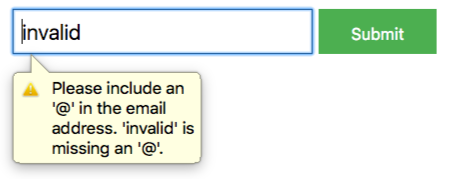
\includegraphics[scale=0.75]{bubi-widget-screenshot}
    \caption{
        \label{fig:bubi-widget-screenshot}
        \texttt{QtWebEngineWidgetUI::MessageBubbleWidget}
    }
\end{figure}

A Qt WebEngine Widgets modulban új widget lett megvalósítva a szövegbuborék számára:
\texttt{MessageBubbleWidget}. Az új widget a \texttt{QtWebEngineWidgetUI} névtérből
elérhető és csak a Qt WebEngine számára. Az új névtér a \texttt{UI Delegate}-ként szolgál
a Qt WebEngine Widgets modulban. Qt WebEngine-hez tartozó \texttt{UI Delegate}-nek fordítási
időben letilthatónak kell lennie, ezért az itt implementált funkciók nem lesznek részei
a Qt WebEngine-nek, ha a projekt a \texttt{WEBENGINE\_CONFIG=no\_ui\_delegates} beállítással
van konfigurálva.

A \texttt{MessageBubbleWidget} singleton-ként van tárolva \texttt{UI Delegate}-en belül,
így nem kell mind üzenethez újra felépíteni a widget-et, csak újra rajzolni. Hozzáférést
az alábbi belső API szolgáltat:
\begin{itemize}
    \item \texttt{QtWebEngineWidgetUI::MessageBubbleWidget::showBubble(} \\
                    \texttt{view, anchor, mainText, subText)}
    \item \texttt{QtWebEngineWidgetUI::MessageBubbleWidget::hideBubble()}
    \item \texttt{QtWebEngineWidgetUI::MessageBubbleWidget::moveBubble(} \\
                    \texttt{view, anchor)}
\end{itemize}
A \texttt{view} (\texttt{QWebEngineView}) paraméterre azért van szükség, hogy a buborék
pozíciója meghatározható legyen az ablakon belül. Az \texttt{anchor} (\texttt{QRect}) annak
a HTML elemnek (beviteli mezőnek) ``körvonala'', amelynek a tartalma a hibát kiváltotta.
Ez arra van használva, hogy a buborék méretét kiszámítsuk. A \texttt{mainText}
(\texttt{QString}) maga a hibaüzenet, míg a \texttt{subText} (\texttt{QString)} HTML mező
azonosítója ha az meg van adva. Maga buborék \texttt{QPainter}-el lett megrajzolva, a bal
felső sarokban található ikon pedig a Qt standard, üzenet mezőhöz tartozó ikonja.

\begin{figure}[ht]
    \centering
    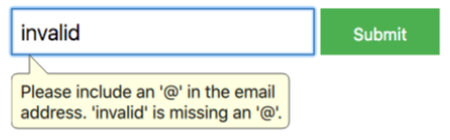
\includegraphics[scale=0.75]{bubi-quick-screenshot}
    \caption{
        \label{fig:bubi-quick-screenshot}
        \texttt{MessageBubble} QML típus
    }
\end{figure}

A Qt WebEngine modul szövegbuborékja mind megvalósítása, mind megjelenítése némileg eltér
a widget-es szövegbuboréktól. A szövegbuborék tárolásáról és annak eléréséről
\texttt{UIDelegatesManager} osztály gondoskodik:
\begin{itemize}
    \item \texttt{UIDelegatesManager:showMessageBubble(} \\
                    \texttt{anchor, mainText, subText}
    \item \texttt{UIDelegatesManager::hideMessageBubble()}
    \item \texttt{UIDelegatesManager::moveMessageBubble(anchor)}
\end{itemize}
A két API többé kevésbé megegyezik. A legfontosabb különbség, hogy itt nem kell átadni a
\texttt{view}-t paraméterül, mert az a \texttt{UIDelegatesManager} adattagja. A szövegbuborék
QML típus QML nyelven lett megvalósítva: \texttt{MessageBubble.qml}. A buborék
megrajzolás a \texttt{Canvas} QML típus segítségével történik. A \texttt{Canvas} típus
ugyanolyan JavaScript API-t nyújt a rajzoláshoz, mint a HTML5 \texttt{Canvas} elem.
Sajnos ikon használatára nem volt lehetőség, mivel a Qt a QML nyelvben nem nyújt beépített
ikonokat sem pedig ikon támogatást. A widget-es ikonok használatát kerülni kellett, mert
a Qt WebEngine modul-nak nem lehet Qt Widgets függősége.

Az Form Validation funkció tesztelésére a Test Support API lett felhasználva. Mivel a
Qt WebEngine-ben a Form Validation-nek nincs publikus API-ja a hiba üzeneteket a
Test Support API teszi elérhetővé a tesztek számára a
\texttt{QQuickWebEngineTestSupport::ValidationMessageShown}
signal-on keresztül. A hibásan kitöltött űrlapok ellenőrzéséhez az elküldés (submit) gomb
megnyomására is szükség van a tesztekben. A teszt a gomb megnyomására felhasználói interakció
híján a Qt Test modul \texttt{keyPress()} függvényét használja. A megfelelő gomb
kiválasztását (``fókuszálását'') JavaScript kód végzi, ahol a megfelelő gomb azonosítóját
az URL fragment tartalmazza.

A Form Validation HTML5 funkció támogatása és a hozzátartozó szöveg buborékok a Qt 5.5-ös
verzióban jelentek meg. A funkció tesztelése már csak az 5.6-os verzióba került be.

\section{Localization}

\begin{center}
    \begin{reviewbox}
        \begin{itemize}
            \renewcommand{\labelitemi}{\textcolor{qtgreen}{$\blacktriangleright$}}
            \item \gerrit{110958}
            \item \gerrit{111004}
        \end{itemize}
    \end{reviewbox}
\end{center}

\noindent
A \textbf{Localization} funkció felel a Chromium üzeneteinek (legyen az hiba üzenet vagy
a Form Validation funkció üzenete) lefordításáért. Alapértelmezetten az üzenetek a
rendszer szinten beállított nyelven fognak megjelenni. Ez a nyelv felüldefiniálható
a render processzben a Chromium \texttt{-{}-lang} kapcsolóval. A browser processzben
ugyanerre a célra a Content API \texttt{ContentBrowserClient::GetApplicationLocale()}
függvényén keresztül van lehetőség.

Tesztelésnél kulcsfontosságú, hogy az üzenetek angol nyelven jelenjenek meg, mivel a
tesztelés során angol nyelvű hiba üzeneteket használjuk referenciaként. A Chromium
alapértelmezett nyelvét a Qt által használt nyelvi beállításokkal definiáltuk felül:
\begin{verbatim}
std::string ContentBrowserClientQt::GetApplicationLocale()
{
    return QLocale().bcp47Name().toStdString();
}
\end{verbatim}
Ez alapján, ahhoz, hogy a tesztekben angol nyelvű hibaüzenetek kapjunk elég a Qt API-n
keresztül beállítani a nyelvet, a tesztelés inicializálásakor:
\begin{verbatim}
QLocale::setDefault(QLocale("en"));
\end{verbatim}
Ez a megoldás azonban nem működött és erről hiba jelentés (bug report) is készült:
\begin{center}
    \begin{issuebox}
        \begin{itemize}
            \renewcommand{\labelitemi}{\textcolor{qtred}{$\blacktriangleright$}}
            \item \qtbug{45715}
        \end{itemize}
    \end{issuebox}
\end{center}

A hiba oka a Chromiumban volt, ezért a javítást a \textit{qtwebengine-chromium} Chromium
forkhoz kellett hozzáadni. A probléma az volt, hogy amelyik rendszeren volt elérhető
GLib ott arra volt bízva a megfelelő lokalizáció kiválasztása. Qt esetében ezt a kód részt
(``code path''-t) ki kellett kapcsolni, hogy ne írja felül a Qt beállításait.

Egyes üzenetek a render processztől jönnek, amelyekre nem érvényes a
\texttt{ContentBrowserClient::GetApplicationLocale} beállítása. A render processznek
és más nem browser processzeknek van egy \texttt{-{}-lang} parancssori kapcsolója, amivel
megadható a kiválasztott locale. A Content API
\texttt{ContentBrowserClientQt::AppendExtraCommandLineSwitches()}
függvényének implementálásával megadható, hogy amikor a browser processz új processzt indít,
annak milyen kapcsolót adjon át. Így ezzel a megoldással minden újonnan induló processznek
átadjuk a \texttt{ContentBrowserClient::GetApplicationLocale()} függvény által visszaadott
locale-t a processz \texttt{-{}-lang} kapcsolóján keresztül:
\begin{verbatim}
AppendSwitchASCII(switches::kLang, GetApplicationLocale());
\end{verbatim}

Ezzel a megoldással a tesztekben kapott Chromium üzenetek minden esetben angolul jelenik meg,
viszont előfordulhat, hogy a felhasználó is szeretné felül definiálni parancssorból a
böngésző alkalmazás nyelvét, ezért a Qt WebEngine-ben a browser processzben is meg lett
valósítva, hogy \texttt{-{}-lang} kapcsolóval átadott érték felülírja a Qt alapértelmezett
nyelvi beállítását. Ez a \texttt{WebEngineLibraryInfo::getApplicationLocale()} függvényben
lett megvalósítva, hogy ha a browser processz \texttt{-{}-lang} kapcsolóval lett indítva,
akkor annak az értékével térjen vissza és ne kérje le a Qt-tól a locale értékét.

Az új \texttt{-{}-lang} parancssori kapcsoló támogatása és a tesztelés javítása a Qt 5.5-ös
verziójában jelent meg.


\section{Authentication Dialog}

\begin{center}
    \begin{reviewbox}
        \begin{itemize}
            \renewcommand{\labelitemi}{\textcolor{qtgreen}{$\blacktriangleright$}}
            \item \gerrit{124330}
            \item \gerrit{124331}
            \item \gerrit{124332}
            \item \gerrit{124333}
        \end{itemize}
    \end{reviewbox}
\end{center}

\noindent
Az legtöbb böngésző támogatja a HTTP protokoll által nyújtott bejelentkezés funkciót
(Basic Access Authentication - RFC 2617), amely a legegyszerűbb módja a web lapok jelszóval
való védésének. Nincs szükség bejelentkező oldalra, cookie-kra, hanem a HTTP header
megfelelő mezőit használja az azonosításhoz. Továbbá HTTP protokoll támogatja a HTTP proxy
szerverre történő bejelentkezést is.

A HTTP protokollon keresztül történő bejelentkezéshez szükséges form (űrlap) nem a web
oldalon jelenik meg, ezért azt jellemzően a böngészők egy felugró ablakon teszik láthatóvá
a felhasználó számára. A Chromium megvalósítja a HTTP protokollon keresztül történő
bejelentkeztetést, viszont a felugró ablakot a beágyazó alkalmazásnak kell megvalósítania
a Content API-n keresztül. A Qt WebEngine ezt megvalósító funkciója az
\textbf{Authentication Dialog}.

Az Authentication Dialog már meg volt valósítva a Qt WebEngine Widgets modulban, azonban
ez a megvalósítás hibás volt, illetve az ehhez tartozó implementáció a Core modulban nem
volt felhasználható egy Quick UI Delegate megvalósításához. A Quick funkció megvalósítását
ezért a Widget API javításával és újraírásával kezdtem.

Az első kijavítandó hiba az volt, hogy a Widget megvalósítás nem támogatta az üres
felhasználónév és jelszó párral történő bejelentkezést, mivel ezt az esetet úgy kezelte,
hogy a felhasználó megszakítja a bejelentkezést (Mégse/Cancel gomb). A felhasználó név
és jelszó (credentials) tárolására a Qt Network module saját osztályt definiál:
\texttt{QAuthenticator}. A hiba javításához megszakítás esetén a \texttt{QAuthenticator}
példány \texttt{user} és \texttt{password} mezőjébe nem üres string-et tárolunk, hanem
nem állítunk be semmit és a példány nem inicializált állapotban marad, amit annak az
\texttt{isNull()} metódusával lehet lekérdezni. Qt Webengine Widgets modul a javításban
ezt az állapotot ellenőrzi és továbbítja a Core modulnak, hogy az azonosítás meg lett e
szakítva vagy sem.

A másik hiba a Widget API-ban a böngésző ikonok (favicon) megjelenítése volt. Amennyiben a
felhasználó jelszóval védett oldalt nyitott meg, bejelentkezés után a böngésző nem tudta
letölteni az oldalhoz tartozó ikont. A probléma oka, hogy az ikon letöltést nem a Chromium
végezte, hanem a Qt Network modul \texttt{QNetworkAccessManager}-re, aminek nem volt
hozzáférése a Chromium által tárolt felhasználónév jelszó pároshoz. A problémát a
Qt WebEngine Widgets module \texttt{demobrowser} példa alkalmazásában kellett orvosolni,
mivel az \texttt{QNetworkAccessManager}-rel támogatott letöltés nem a Qt WebEngine API része.
A javítás ezért egy ideiglenes ``workaround'' lett, amíg az ikonok letöltésért felelős
funkcionalitás/API nincs megvalósítva a Qt WebEngine-ben. A javítás lényege az, hogy a
legutóbbi Authentication Dialog-ban bevitt felhasználónév/jelszó párost hordozó
\texttt{QAuthenticator} példányt a böngésző oldalon is tároljuk és amikor a
\texttt{QNetworkAccessManager} azonosítást igényel, akkor a tárolt a adatokkal próbálja
azonosítani magát.

Ennél a javításnál különösen kellett ügyelni arra, hogy ez a workaround ne adjon lehetőséget
visszaélésre, például az eltárolt adatok megszerzésére egy kimondottan erre a célra
készített web oldal betöltésével. A támadások kivédésére a \texttt{QAuthenticator} példány
tárol a web oldalhoz vagy a proxy szerverhez tartozó információkat is azok egyértelmű
azonosításához. Így a \texttt{QNetworkAccessManager} csak olyan lekérésnél próbál meg
bejelentkezni a \texttt{QAuthenticator}-ban tárolt adatokkal, ahol az azonosítást kérő
szervert egyértelműen azonosítani tudja. További szépséghibája a javításnak, hogy
ugyanezt a problémát a QML/Quick API-ra építő böngészőkben nem oldja meg, mivel ott az ikon
letöltése az \texttt{Image} QML típuson történik, amely nem nyújt lehetőséget az
autentikációra.

Widget hibák javítása után a következő akadályt a Quick API Authentication Dialog-jának
megvalósításához a Content API \texttt{ResourceDispatcherHostLoginDelegate} interfészének
implementációja jelentette. Ez az interfész már meg volt valósítva az egyszerűség kedvéért
a Widget ``szinkron'' API-jának megfelelően. A szinkron API ez esetben azt jelenti, hogy a
\texttt{QWebEnginePrivate::authenticationRequired()} függvényen belül kiküldött
\texttt{authenticationRequired} vagy \texttt{proxyAuthenticationRequired} szignálok által
kiváltott slot-ok (ez esetben a dialog) végrehajtását a függvény megvárja és nem megy tovább,
így nem kell a dialog ablak bezárását külön eseménnyel lekezelni. A Quick aszinkron API-jával
ez nem megoldható, ezért a \texttt{ResourceDispatcherHostLoginDelegate}-nek olyan közös
megvalósítására van szükség a Core modulban, amely mind két típusú API-val használható.

A új közös belső Core API-t \texttt{AuthenticationDialogController} osztály valósítja meg
a hasonló \texttt{JavaScriptDialogController} osztály mintájára.
Az \texttt{AuthenticationDialogController} osztály a
\texttt{ResourceDispatcherHostLoginDelegateQt} példányosítja, amikor a Content API jelez,
hogy új Authentication Dialog ablakra van szükség. Példányosítás után a
\texttt{ResourceDispatcherHostLoginDelegateQt} átadja azt az API-nak, hogy azon keresztül
az beállíthassa a felhasználótól bekért felhasználónév/jelszó párost.

Az \texttt{AuthenticationDialogController}-en
belül két slot van megvalósítva: \texttt{accept()} a belépéshez és \texttt{reject()} a
megszakításhoz. A slotok implementálják Chromium értesítését a Content API-n keresztül a
felhasználói interakció eredményéről. A Widget API könnyen hozzáigazítható volt az új
modellhez és hála a két új slot-nak a \texttt{AuthenticationDialogController} alkalmas
olyan aszinkron API megvalósítására is mint a Qt WebEngine modul, Quick API-ja.

Amíg a Widget API-ban lehetséges a fejlesztőre bízni a dialog megvalósítását, addig a
QML/Quick API-ban (még) nincs lehetőség saját dialog ablakok összekötésére a Qt WebEngine
eseményeivel. Ezért a Quick Authentication Dialog-ot Qt WebEngine-en belül kellett
megvalósítani \texttt{UIDelegatesManager} segítségével akár csak a Form Validation funkció
szöveg buborékja (\texttt{MessageBubble}) esetén.

Mivel a Qt Declarative komponens nem nyújt bejelentkező (login) dialog ablakot a Quick-hez,
ezért nem volt elég egy már meglévő QML típust bekötni a \texttt{UIDelegatesManager}-be,
hanem egy újat kellett implementálni erre a célra QML nyelven:
\texttt{AuthenticationDialog.qml}. Ez az új QML típus csak a QtWebEngine-ből használható,
a publikus API-n keresztül nem érhető el. A dialog ablak üzenetei és az események lekezelése
a \texttt{UIDelegatesManager}-en belül vannak megvalósítva C++ nyelven.

\begin{figure}[ht]
    \centering
    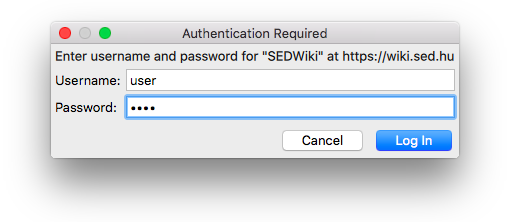
\includegraphics[scale=0.75]{ad-quick-screenshot}
    \caption{
        \label{fig:ad-quick-screenshot}
        \texttt{AuthenticationDialog} QML típus
    }
\end{figure}

A javítások és az új Quick Authentication Dialog ablak a Qt 5.6-os verziójában jelentek meg.


\section{Favicon Manager}

\noindent
A \textbf{favicon} a web oldalhoz tartozó ikon, vagy más néven \textit{shortcut icon}. A
favicon-t web oldal HTML kódjában kell megadni az alábbi módon:
\begin{verbatim}
<html>
    <head>
        <link rel="shortcut icon" href="favicon.png" />
    </head>
</html>
\end{verbatim}
A böngészőalkalmazás ezt az ikont tetszőleges célokra használhatja fel, jellemzően az URL
bar-on vagy a tab-on jelenítik meg.
Az oldalhoz rendelt ikon lehet \textit{touch icon} is. A touch icon többnyire nagyobb
felbontású, mint a favicon és elsősorban érintőképernyős készülékeken használják az
előzmények és/vagy könyvjelzők megjelenítésére. Egy oldalhoz több favicon és/vagy touch icon
is tartozhat, böngészőalkalmazás feladata választani közülük.

A Qt WebEngine-ben megvalósított \textbf{Favicon Manager} ezeket az ikonokat tölti le a
Chromium Content API-n keresztül, tárolja azokat és implementál belső API-t az elérésükre.
Megvalósítását több cél is motiválta:
\begin{itemize}
    \item Az jelszóval védett oldalak betöltése esetén ne legyen szükség workaround-ra a
        böngészőalkalmazás kódjában ahhoz, hogy le lehessen tölteni egy ikont
    \item A Qt WebEngine korábbi verziói nem támogatták a touch icon-ok használatát
    \item A Qt WebEngine korábbi verziói nem támogatták az ikonok közötti választást
    \item Bizonyos esetekben a touch icon-ok közül is a legnagyobb felbontásúra van szükség
\end{itemize}

Mivel a Favicon Manager megvalósítása sok részfeladatot foglal magában, ezért ezek
rendszerezésére egy gyűjtő issue-t készítettem:
\begin{center}
    \begin{issuebox}
        \begin{itemize}
            \renewcommand{\labelitemi}{\textcolor{qtred}{$\blacktriangleright$}}
            \item \qtbug{51179}
        \end{itemize}
    \end{issuebox}
\end{center}
Ebben a fejezetben felsorolt patch-ek egy-egy részfeladatot valósítanak meg. Egy részük
új funkciót vezetnek meg, míg mások hiba javításokat vagy teszteket tartalmaznak.

\begin{center}
    \begin{reviewbox}
        \begin{itemize}
            \renewcommand{\labelitemi}{\textcolor{qtgreen}{$\blacktriangleright$}}
            \item \gerrit{127480}
            \item \gerrit{148542}
        \end{itemize}
    \end{reviewbox}
\end{center}

Az új funkció alapját a WebEngine Core modulban implementált \texttt{FaviconManager} osztály
valósítja meg. Ez az osztály tölti le a megjelenített oldalhoz tartozó ikonokat,
választja ki közülük a megfelelőt, jelez a publikus API-nak ha a view-hoz rendelt ikon
megváltozott, a publikus API ezen keresztül tudja lekérni az ikont.
A kódban már a C++11 szabvány \textit{range-based for} nyelvi elemét használtam fel az
iterációkhoz az optimális megvalósítás érdekében.

Az ikonok letöltéséhez a Content API \texttt{WebContents::DownloadImage()} függvényét
használom, ezáltal nincs szükség külön implementációra az autentikációhoz, azt a Content API
elvégzi. Abban az esetben, ha az ikon QRC-ben (Qt Resource System)\footnote{A Qt ezen
    funkciójával teszi azt lehetővé, hogy a Qt-s alkalmazáshoz tartozó fájlokat a
    binárison belül tároljuk. A Chromium nem támogatja ezt a protokollt.}
van tárolva, az ikon betöltése Qt API-n keresztül történik, nincs szükség letöltésre.

A Favicon Manager a web oldalhoz tartozó összes ikont megpróbálja letölteni és azokat egy
\texttt{QMap}-ben tárolja. A map-ből az ikont az URL-je alapján lehet elérni. A Favicon
Manager letöltés előtt ellenőrzi, hogy a map-ben benne van e már az ikon, ha benne van,
nem ismétli meg a letöltést, így gyorsítótárazva (cache) az ikonokat.

Minden tabhoz (WebEngineView-hoz) saját Favicon Manager tartozik, ezért előfordulhat, egy
bizonyos ikon többször van tárolva a memóriában. Ennek a modellnek az előnye a gyorsabb
keresés és az egyszerűbb implementáció. A publikus WebEngineView API a
\texttt{iconChanged()} signal-al jelzi, hogy ha megváltozott a view-hoz tartozó ikon.
Ez az ikon a publikus API-n keresztül lekérhető (\texttt{icon} és \texttt{iconUrl}
property-k), az API pedig a Favicon Manager-től kéri el.
A Favicon Manager a letöltött ikonok közül a legnagyobb felbontásút fogja felajánlani.

A publikus API-k közvetlenül nem változtak, viszont működésük némileg igen. Így indokolttá
vált a Quick és Widget API-k favicon tesztjeinek kibővítése és lefedettségük növelése, ami
az első Favicon Manager-t megvalósító patch jelentős részét teszi ki.

\begin{center}
    \begin{reviewbox}
        \begin{itemize}
            \renewcommand{\labelitemi}{\textcolor{qtgreen}{$\blacktriangleright$}}
            \item \gerrit{150667}
            \item \gerrit{150668}
            \item \gerrit{153438}
        \end{itemize}
    \end{reviewbox}
\end{center}

A publikus Favicon Manager publikus API-jának fejlesztése során több változat is született.
Végül úgy döntöttünk, hogy az 5.7-es verzióban nem lesz a Favicon Manager-nek publikus
API-ja, hanem a már meglévő ikon API-k lesznek tovább fejlesztve. Habár a tervezett
funkcionalitások még bevezetésre kerülhetnek a Qt 5.8-as verziójában, karbantarthatóság
miatt az ezt támogató WebEngine Core-ban implementált funkciókat eltávolítottam.
A Favicon Manager implementációjának karbantartása mellett, a fejlesztés közben megtalált
hibákat is javítottam.

\begin{center}
    \begin{reviewbox}
        \begin{itemize}
            \renewcommand{\labelitemi}{\textcolor{qtgreen}{$\blacktriangleright$}}
            \item \gerrit{151057}
        \end{itemize}
    \end{reviewbox}
\end{center}

Habár új publikus API-t nem vezettünk be a Favicon Manager-hez, mindenképpen szerettem volna,
hogy ha a fejlesztőnek van kontrollja az ikonok letöltése felett. Ennek megvalósításához
a \texttt{WebEngineSettings}-hez adtam hozzá új beállításokat:
\begin{description}
    \item[\texttt{AutoLoadIconsForPage}] Az ikonok automatikusan legyenek letöltve
    \item[\texttt{TouchIconsEnabled}] Legyenek letiltva a touch ikonok is
\end{description}

A \texttt{AutoLoadIconsForPage} beállítás alapértelmezetten engedélyezve van, letiltásával
a Qt WebEngine nem tölti le az ikonokat, ezáltal a böngészőalkalmazás gyorsabb lehet,
spórolhat a sávszélességen, továbbá a fejlesztőnek van lehetősége saját ikon manager-t
implementálni úgy, hogy ne kelljen törődnie a Qt WebEngine API ikon signal-jaival.

A \texttt{TouchIconsEnabled} beállítás desktop környezetben alapértelmezetten le van tiltva.
Egy klasszikus desktop böngészőalkalmazásnak nincs szüksége touch ikonokra.

\begin{center}
    \begin{reviewbox}
        \begin{itemize}
            \renewcommand{\labelitemi}{\textcolor{qtgreen}{$\blacktriangleright$}}
            \item \gerrit{151314}
            \item \gerrit{151315}
            \item \gerrit{157142}
        \end{itemize}
    \end{reviewbox}
\end{center}

Önmagában a Favicon Manager megvalósítása a WebEngine Core modulban nem sok előnyt nyújt.
Szükséges a publikus API-k módosítása is, hogy kihasználják a Favicon Manager által nyújtott
lehetőségeket. Az API-k bővítését a Widget API-val kezdtem, mivel annak megvalósítása
egyszerűbb és a WebEngine Widgets modulra épülő demobrowser-ben a Favicon Manager haszna
jól demonstrálható.

A WebEngineWidgets module két API-t is nyújt az ikonok elérésére. Az egyik a
\texttt{QWebEnginePage}, a másik a \texttt{QWebEngineView}. A kettő lényegében ugyanaz:
a \texttt{QWebEnginePage} \texttt{iconUrl} property-jén keresztül elérhető a page-hez
tartozó ikon URL-je, amennyiben ez az URL megváltozik akkor egy \texttt{iconUrlChanged}
signal-t küld. A \texttt{QWebEngineView} ugyanezt a property-t és a hozzátartozó signal-t
valósítja meg, csak az éppen megjelenített page-hez tartozó URL-t adja vissza.

Az API-k egy új \texttt{icon} property-vel és a hozzátartozó \texttt{iconChanged} signal-al
lettek bővítve. Az új property a már meglévő \texttt{iconUrl} property-hez hasonlóan működik,
azzal az eltéréssel, hogy nem az ikon URL-jét tartalmazza, hanem az URL-ről letöltött ikont
egy \texttt{QIcon} példányban tárolva. Az új property-nek hála a böngészőalkalmazásnak nem
kell megvalósítania a letöltést, így a demobrowser példa böngészőalkalmazásból is
eltávolítottam a \texttt{QNetworkAccessManager} használatát és az autentikációhoz szükséges
workaround-ot is.

Az bővített API-val most már a WebEngine Widgets modul támogatja az olyan ikonok használatát
is, amelyek több különböző méretű ikont ágyaznak magukba (\textit{multi-size icon}).
Ezekhez, és az új \texttt{icon} property-hez teszteket is készítettem,
a \texttt{QWebEnginePage} és \texttt{QWebEngineView} API-k dokumentációit bővítettem és
naprakésszé tettem.

\begin{center}
    \begin{reviewbox}
        \begin{itemize}
            \renewcommand{\labelitemi}{\textcolor{qtgreen}{$\blacktriangleright$}}
            \item \gerrit{154018}
            \item \gerrit{156213}
        \end{itemize}
    \end{reviewbox}
\end{center}

A WebEngine QML API esetében a Widget-hez hasonló bővítés megvalósítás sokkal bonyolultabb
volt, mivel sem a QML, sem a Quick nem nyújt ikon támogatást. Az ikon megjelenítésére az
\texttt{Image} QML típus használható, viszont annak az API-ja csak URL alapján tud képet
betölteni. A Favicon Manager a letöltött ikont a memóriában tárolja és nem érhető el URL-el.

Erre a problémára megoldást a Quick API \texttt{QQuickImageProvider} interface-e nyújt
megoldást. A QML contextben beregisztrált image provider egy speciális URL-el rendelkezik,
ha az \texttt{Image} QML típus egy ilyen URL-t kap forrásként, akkor a kérést a provider-hez
irányítja, amely betölti az \texttt{Image}-be a megfelelő képet.

Az új \texttt{QQuickWebEngineFaviconProvider} osztály ezt az osztályt valósítja meg.
Amennyiben az \texttt{Image} forrás URL-je \texttt{image://favicon/url} alakú, akkor a
kérést a \texttt{QQuickWebEngineFaviconProvider}-hez irányítja, amely elkéri a
Favicon Manager-től a \texttt{url}-hez bejegyzett ikont. A \texttt{Image} rendelkezik
egy \texttt{sourceSize} property-vel is, amelynek értékét a provider megkapja, így ezt a
multi-size ikonok támogatására használtam fel. Amennyiben az URL-ben hivatkozott ikon
multi-size és a \texttt{sourceSize} be van állítva, akkor a \texttt{sourceSize}-ban definiált
mérethez legjobban illeszkedő ikont tölti be a \texttt{QQuickWebEngineFaviconProvider}.

Az új provider használatához módosítani kellett a \texttt{WebEngineView} QML típus
\texttt{icon} property-jét. Ez a property korábban az ikon eredeti URL-jét tárolta,
az új módosítással a property-ben tárolt URL a \texttt{QQuickWebEngineFaviconProvider}
speciális URL-je, amelyen keresztül elérhető a Favicon Manager-ben tárolt ikon.

A \texttt{QQuickWebEngineFaviconProvider} tesztelése külön kihívást jelentett számomra.
Mindenképpen azt szerettem volna tesztelni, hogy a provider a \texttt{sourceSize}-nak
megfelelő ikont tölti-e be. A teszt stratégiám az volt, hogy minden tesztelni kívánt mérethez
egy szürke árnyalatos ikont készítek, és ezekből egy multi-size ikont generálok. Az egyes
szürke árnyalatos ikonok az RGB színcsatornáikban a saját méretüket kódolják. Például, a
32x32-es méretű ikonnak minden pixelének RGB értéke (32, 32, 32). Teszt betöltött ikon
egy pixelének, egyik színcsatornájának értékét vizsgálja meg, hogy megegyezik-e
a \texttt{Image} QML típus \texttt{sourceSize} property-jénék értékével.

A teszt megvalósításánál a legnagyobb problémát az okozta, hogy a \texttt{Image} QML
típus nem nyújt API-t a pixelek lekérdezésére. QML-ben erre a \texttt{Canvas} típusban
van lehetőség, amely ugyan tud képet betölteni provider-ből, viszont támogat
\texttt{sourceSize} vagy ahhoz hasonló property. Ennek a problémának a megoldására egy
sor workaround-ra volt szükség, de végül sikerült a betöltött ikon egy pixelét QML és
JavaScript kóddal lekérdezni. Ezen speciális teszt megvalósítása során sikerült a
Qt Declarative komponens Quick moduljában is hibát találni, amit ki is javítottam.

\begin{center}
    \begin{reviewbox}
        \begin{itemize}
            \renewcommand{\labelitemi}{\textcolor{qtgreen}{$\blacktriangleright$}}
            \item \gerrit{155559}
        \end{itemize}
    \end{reviewbox}
\end{center}

Mivel sikerült a Qt WebEngine Quick és Widget API-jait úgy bővíteni, hogy képesek legyenek
támogatni a multi-size ikonokat, így kompromisszumos megoldásnak tűnt külön Favicon Manager
API helyett ezt a funkciót felhasználni arra, hogy egy adott oldalhoz elérhető ikonok
(\textit{candidate icons}) listájából válogatni lehessen.

A megvalósításban a Favicon Manager a candidate ikonokat egy multi-size ikonba gyűjti össze.
Azonos méretű ikonok esetén csak az marad bent, amelyik először került bele a multi-size
ikonba. Amikor a böngészőalkalmazás lekéri az ikont a WebEngine-től akkor ezt az ikont
fogja megkapni. Az ikon méretezésének megfelelően a méretben legmegfelelőbb ikon kerül
betöltésre.

A Widget API esetében a méretezést a \texttt{QIcon} API-ján keresztül történik, míg a
Quick API esetén a \texttt{QQuickWebEngineFaviconProvider}-en keresztül a már leírtak
szerint. Ebből kifolyólag a tesztelés is hasonlóan történik, mint a multi-size ikonok
esetén.

\begin{center}
    \begin{reviewbox}
        \begin{itemize}
            \renewcommand{\labelitemi}{\textcolor{qtgreen}{$\blacktriangleright$}}
            \item \gerrit{156064}
        \end{itemize}
    \end{reviewbox}
\end{center}

Böngészőkben az ikonokkal nem csak az éppen látható oldalt azonosíthatjuk, hanem a már
látogatottakat is. A Quick API-ban korábban nem volt lehetőség a böngészési előzményekhez
rendelt ikonokhoz hozzáférni. A továbbfejlesztett Navigation History API-ban már elérhető
az előzményekhez rendelt \texttt{QQuickWebEngineFaviconProvider} specifikus URL.

A fejezetben bemutatott Favicon Manager és az ahhoz kapcsolódó API fejlesztések a Qt 5.7-es
verziójában fognak megjelenni. A Favicon Manager publikus API-jának elkészítése tervben van,
az leghamarabb a Qt 5.8-as verziójában jelenhet meg, ha úgy döntünk, hogy szükség van rá.
További terv az 5.8-as verzióba, egy ikon adatbázis megvalósítása, ami a QtWebKitnek is
része. Az adatbázis segítségével az ikonok lemezre menthetőek lennének és ezáltal offline
módban is hozzáférhetőek. A tervről issue is készült:
\begin{center}
    \begin{issuebox}
        \begin{itemize}
            \renewcommand{\labelitemi}{\textcolor{qtred}{$\blacktriangleright$}}
            \item \qtbug{51184}
        \end{itemize}
    \end{issuebox}
\end{center}


\chapter{Egy példa böngészőalkalmazás megvalósítása}

A \ref{chap:features}. fejezetben bemutatott új funkciók használatát egy saját
böngészőalkalmazás segítségével mutatom be ebben a fejezetben. Az alkalmazást első sorban
desktop környezetre szántam. Mivel a Qt egy cross-platform keretrendszer így a példa
böngészőalkalmazás működik a legnépszerűbb desktop operációs rendszereken: Windows, Linux,
OS X. Mindemellett elméletileg működik beágyazott környezetben is (pl.: Embedded Linux),
ahol a Qt WebEngine támogatott (Androidon már nem), viszont ez nem került kipróbálásra.

Az alkalmazást QML nyelven valósítottam meg. Minimális C++ kód is része a megvalósításnak,
amely két részből áll. Az egyik a program fő belépési pontjának megvalósítása, amely
inicializálja a Qt WebEngine OpenGL és QML környezetét, illetve betölti a QML programot:
\begin{lstlisting}[title=main.cpp]
 int main(int argc, char *argv[])
 {
    QApplication app(argc, argv);

    QtWebEngine::initialize();

    QQmlApplicationEngine engine;
    Utils utils;
    engine.rootContext()->setContextProperty("utils", &utils);
    engine.load(QUrl(QStringLiteral("qrc:/main.qml")));

    return app.exec();
 }
\end{lstlisting}
A másik rész segédfüggvényeket implementál a QML nyelvhez, amelyek a \texttt{utils} propertyn
elérhetőek QML-ből. A segédfüggvények az alábbiak:
\begin{description}
    \item[\texttt{fromUserInput(userInput)}] A paraméterül kapott stringet URL-é alakítja
        annak megfelelően, hogy a hivatkozott erőforrás lokálisan vagy HTTP protokollon
        keresztül érhető el
    \item[\texttt{setLocale(locale)}] A Qt alapértelmezett nyelvi beállításait definiálja
        felül a \texttt{locale} paraméterrel
\end{description}

\section{Felhasználói felület (GUI)}

A QML kód túlnyomó része a GUI-t valósítja meg. Mivel a QML egy deklaratív nyelv, nem kellett
túl sokat dolgozni a működés megvalósításán, azt a Qt WebEngine Quick/QML API-ja már
megvalósította. A hangsúly a megjelenés megtervezésén van, ezért könnyű a QML nyelven
programozni, a fejlesztőnek csak a GUI elemek testre szabására és az azok közötti
interakciókra kell figyelni. Lényegében a \texttt{WebEngineView} QML típus is egy GUI elem,
ami a web oldal tartalmát rajzolja egy téglalap alakú felületre és küld értesítést
(signal-okat) a nézetben történt változásokról.

A GUI megtervezésénél legfőbb szempontnak tartottam, hogy a böngészőalkalmazás desktop-ra
készül, ahol a megjelenítő szélessége nagyobb, mint a magassága. Ezzel szemben a web oldalak
általában magasabbak, mint szélesek, ezért a bal szélen ki nem használt területet a tabok
és a böngészési előzmények megjelenítésére használtam fel. A másik fontos szempont az volt,
hogy az alkalmazás ablakának minél nagyobb részét a böngészési felület
(\texttt{WebEngineView}) töltse ki. Ezt elsősorban animált, nyitható-csukható panelek
megvalósításával próbáltam elérni.

A böngészőalkalmazás megjelenését igyekeztem minél egyedibbé tenni, ezért a QML megvalósítás
több új, saját QML típust is tartalmaz. Ezek az új típusok (GUI elemek), ahol csak lehet
kihasználják a Quick keretrendszer által nyújtotta előnyöket: az elemek tulajdonságai
(méret, pozíció, szín, stb) dinamikusan változnak, az átmenetek animálva vannak, hogy
egy valódi "fluid" felületté álljanak össze.

\subsection{Vezérlők (controls)}
A legalapvetőbb ilyen elemek, amelyek valamilyen felhasználói interakcióra (első sorban
bal gombbal kattintásra) adnak választ. Ilyen vezérlő elemeket Qt QuickControls modulja
is tartalmaz, melyeket sok helyen fel is használtam. Néhány elemet azonban magam valósítottam
meg, hogy jobban illeszkedjenek a tervezett GUI-ba.

\subsubsection{Gombok}
Háromféle különböző gombot használtam fel, amelyek egy közös őstől származnak,
a saját \texttt{Button} QML típusból. A gombok működésben nem térnek el egymástól csak a
színezésük más. Egy gombnak négy állapota lehet:
\begin{description}
    \item[\texttt{released}] Alapállapot
    \item[\texttt{disabled}] A gomb le van tiltva, nem reagál felhasználói interakcióra
    \item[\texttt{hovered}] Az egérmutató a gomb felett van
    \item[\texttt{pressed}] Bal egérgombot lenyomva tartjuk a gomb felett
\end{description}

A \ref{fig:browser-button}, \ref{fig:settings-button} és \ref{fig:close-button} ábrák
mutatják be a felhasznált gombokat, rendre azok lehetséges állapotaikkal együtt.

\begin{figure}[H]
    \centering
    
\includegraphics[scale=0.8]{BrowserButton}
    \caption{
        \label{fig:browser-button}
        \texttt{BrowserButton} 4 állapota: \textit{released}, \textit{disabled},
        \textit{hovered} és \textit{pressed}
    }
\end{figure}
\begin{figure}[H]
    \centering
    
\includegraphics[scale=0.8]{SettingsButton}
    \caption{
        \label{fig:settings-button}
        \texttt{SettingsButton} 4 állapota: \textit{released}, \textit{disabled},
        \textit{hovered} és \textit{pressed}
    }
\end{figure}
\begin{figure}[H]
    \centering
    
\includegraphics[scale=0.8]{CloseButton}
    \caption{
        \label{fig:close-button}
        \texttt{CloseButton} 4 állapota: \textit{released}, \textit{disabled},
        \textit{hovered} és \textit{pressed}
    }
\end{figure}


\subsubsection{Kapcsoló}
A \texttt{BrowserSwitch} QML típus egy két állapotú kapcsolót valósít meg. Csak egy helyen
van felhasználva, viszont általánosan van megvalósítva, hogy újra felhasználható legyen.

\begin{figure}[H]
    \centering
    %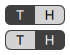
\includegraphics[scale=0.8]{BrowserSwitch-compact}
    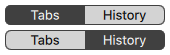
\includegraphics[scale=0.8]{BrowserSwitch-wide}
    \caption{
        \label{fig:browser-switch}
        \texttt{BrowserSwitch} 2 állapota: fent bal oldal, lent jobb oldal van kiválasztva
    }
\end{figure}

\subsubsection{Lista elem sablonok}
\label{sec:list-entry-templates}
A tabok és a böngészési előzmények listáját a \texttt{ListView} QML típus valósítja mag.
A \texttt{ListView} típus az elemeket egy sablon QML típus példányosításával
jeleníti meg. Ilyen saját template típusok a \texttt{CompactEntry} és a \texttt{WideEntry}.
\begin{figure}[H]
    \centering
    
\includegraphics[scale=0.8]{Compact-Wide-Entries}
    \caption{
        \label{fig:compact-wide-entries}
        \texttt{CompactEntry} felül és \texttt{WideEntry} alul
    }
\end{figure}
A \texttt{CompactEntry} csak a weboldal ikonját jeleníti meg nagy méretben (touch ikont, ha
van elérhető). A \texttt{WideEntry} szélessége miatt nagyobb helyet foglal, megjeleníti az
oldal kis méretű favicon-ját, mellette pedig a web oldal címét. Ezek a lista elem sablonok
tulajdonképpen nem ``vezérlők'', mert a felhasználói eseményeket nem az elem, hanem a
\texttt{ListView} QML típus kezeli le, viszont a felhasználó a lista elemre kattintva
``vezérli'' az alkalmazást.

\subsection{Nézetek (views)}
Ebbe a kategóriába olyan saját QML típusokat sorolok, amelyek más GUI elemeket fognak össze
és jelenítenek meg a nézet típusa szerint.

\subsubsection{Lista nézetek}
A \ref{sec:list-entry-templates} alfejezetben már volt arról szó, hogy a példa
böngészőalkalmazás saját sablonokat használ lista elemek létrehozására. A listák
megjelenítésére a \texttt{ListView} QML típus saját, specializált változatait használja:
\texttt{TabListView}-t a tabokhoz és \texttt{HistoryListView}-t a böngészési előzményekhez.
\begin{figure}[H]
    \centering
    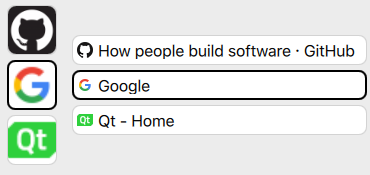
\includegraphics[scale=0.5]{TabListView}
    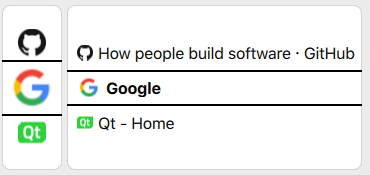
\includegraphics[scale=0.5]{HistoryListView}
    \caption{
        \label{fig:tab-list-view}
        \texttt{TabListView} és \texttt{HistoryListView}
    }
\end{figure}

\subsubsection{SliderPanel}
A \texttt{SliderPanel} egy olyan felület, amivel a GUI nem gyakran használt elemeit rejthetjük
el, vagy kicsinyítjük le a nagyobb helykihasználás érdekében. A lista nézetek esetén a
\textit{Wide} és \textit{Compact} mód közötti váltás is \texttt{SliderPanel} segítségével
történik. Ez a QML típus testre szabható, hogy vízszintesen vagy függőlegesen jelenjen meg,
illetve, hogy teljesen vagy csak részben csukódjon össze.
\begin{figure}[H]
    \centering
    
\includegraphics[scale=0.8]{SliderPanel}
    \caption{
        \label{fig:slider-panel}
        \texttt{SliderPanel} zárt és nyitott állapotban
    }
\end{figure}

\subsubsection{SettingsPanel}
A \texttt{SettingsPanel} egy dialógus ablakot megvalósító saját QML típus. A panel
mozgatható (\textit{drag}), a bezárás és az Ok gombok (\texttt{SettingsButton}) a típus
részei, beépített \textit{confirm dialog}-gal rendelkezik, a vezérlő elemek bővíthetőek
és a tartalom görgethető. A \texttt{SettingsPanel} saját stílus definíciókat is tartalmaz
a \texttt{Checkbox} és \texttt{TextField} QML típusokhoz.

\begin{figure}[H]
    \centering
    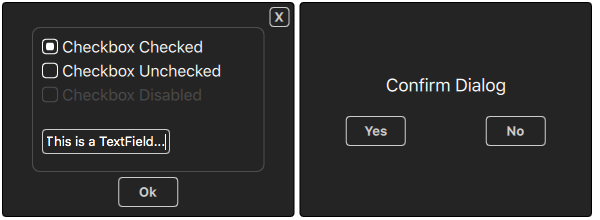
\includegraphics[scale=0.7]{SettingsPanel}
    \caption{
        \label{fig:settings-panel}
        \texttt{SettingsPanel} beállításokkal és a beépített confirm dialog-gal
    }
\end{figure}

\subsection{QtWebEngine specifikus QML típusok}
Az alábbi típusok a nézetekhez hasonlóak, de nem általánosan újra felhasználhatóak.
Tartalmuk rögzített, melyek felhasználják a \texttt{WebEngineView} QML típus valamely
property-jét.

Az \texttt{AddressBar} típus a betölteni kívánt weboldal URL-jének megadására használatos.
Ez a GUI eleme interaktív, mutatja az oldal betöltésének állapotát és az oldal favicon-ját
teljesen betöltött oldal esetén.
\begin{figure}[H]
    \centering
    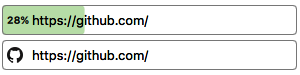
\includegraphics[scale=0.8]{AddressBar}
    \caption{
        \label{fig:address-bar}
        \texttt{AddressBar} oldal betöltés közben és betöltött oldallal
    }
\end{figure}

A \texttt{FindBar} típus kifejezetten a Qt WebEngine Find Text funkciójának használatára
lett létrehozva. Tartalmaz egy szövegmezőt a keresendő szöveg beviteléhez, gombokat
(\texttt{BrowserButton}) a találatok navigációjához és egy bezáró gombot
(\texttt{CloseButton}) a keresés alapállapotba állításához és a \texttt{FindBar}
elrejtéséhez.
\begin{figure}[H]
    \centering
    
\includegraphics[scale=0.8]{FindBar}
    \caption{
        \label{fig:find-bar}
        \texttt{FindBar}
    }
\end{figure}

\subsection{Modellek (models)}
A példa böngészőalkalmazáshoz megvalósított saját modellek valójában nem GUI része, mert
nem megjelenést definiálnak. Dinamikus tartalmat határoznak meg, amelyet más QML típusoknak
kell megjeleníteniük. A megvalósítások a \texttt{ListModel} QML típust specializálják úgy,
hogy tartalmuk egyedi módon változtatható legyen.

\subsubsection{WebEngineViewListModel}
Ez a modell az alkalmazás egyik legfontosabb eleme. Új \texttt{WebEngineView} példányok
ezen keresztül hozhatóak létre, szúrhatóak be listába, távolíthatóak el a már nem
szükséges példányok. A \texttt{TabListView} saját QML típus ennek a modellnek az elemeit
jeleníti meg.

\subsubsection{LocaleListModel}
A \texttt{LocaleListModel} tartalmazza a böngészőalkalmazás által beállítható nyelvek
listáját. Néhány nyelv a modellben előre meg van adva, példányosításkor a listába
kerül a futtató rendszer alapértelmezett nyelve is. Ezt a modellt a
\texttt{SettingsPanel}-en található, nyelv kiválasztó \texttt{ComboBox} QML típus használja.

\subsection{Összkép}
A saját és a Qt gyári QML típusai a \texttt{main.qml} QML fájlban vannak példányosítva és
összekötve. Ez az alkalmazás QML megvalósításának fő belépési pontja, amely egy
\texttt{ApplicationWindow} QML típusban helyezi el a GUI elemeket.

\begin{figure}[H]
    \centering
    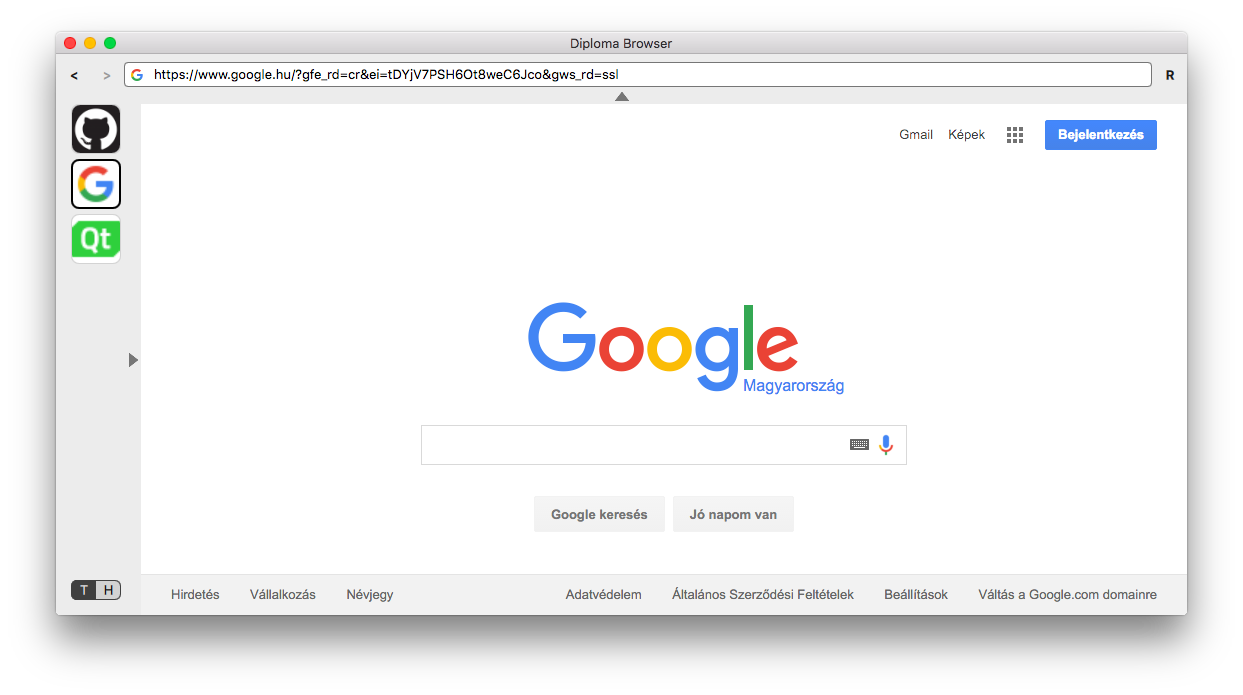
\includegraphics[scale=0.34]{diplomabrowser}
    \caption{
        \label{fig:diplomabrowser}
        A példa böngészőalkalmazás képernyőképe
    }
\end{figure}

\newpage
\section{Az új QtWebEngine funkciók használata}

Az funkciók használatának bemutatására a példa böngészőalkalmazás QML kódját használom fel.
A legtöbb esetben a példakód nem egy-egy az egyben lett bemásolva, hogy az olvashatóbb
legyen és nyomtatásban kiférjen. Minden kódrészletnél megjelöltem, hogy az eredeti
melyik forrásfájlban található. Eltávolításra kerültek még a funkcióhoz nem kapcsolódó
kódrészletek is, hogy azok ne legyenek zavaróak vagy félrevezetőek a magyarázatban.

\subsection{Favicon Manager}

A példa alkalmazásban az ikonokat minden esetben a \texttt{Image} QML típussal jelenítem meg.
Ikonok összesen három saját QML típusban fordulnak elő: \texttt{AddressBar},
\texttt{CompactEntry} és \texttt{WideEntry}. Az API használata lényegében nem tér el a három
típusban, ezért azt az \texttt{AddressBar} kódjával szemléltetem:
\begin{lstlisting}[title=AddressBar.qml]
 Image {
    id: icon

    width: 16; height: 16
    sourceSize: Qt.size(width, height)
    source: root.iconUrl
    /* ... */
 }
\end{lstlisting}
A Favicon Manager szempontjából két property fontos: a \texttt{sourceSize} és a
\texttt{source}. A \texttt{sourceSize} property mondja meg, hogy mekkora ikont kell
betöltenie a Favicon Provider-nek. Jelen esetben ez úgy van megadva, hogy egyezzen meg az
\texttt{Image} elem méretével, így az ha dinamikusan változik, akkor a Favicon Provider
implicit az új méretnek megfelelő ikont tölti be.

A \texttt{source} property értékének egy, a Favicon Provider-re hivatkozó URL-nek kell lennie.
Ezt az URL-t a \texttt{WebEngineView::icon} property tárolja. Azért, hogy az
\texttt{AddressBar} típusnak ne kelljen beimportálnia a Qt WebEngine modult, ezért a saját
\texttt{iconUrl} property-jén keresztül éri el az URL-t. Az \texttt{iconUrl} property-nek az
\texttt{AddressBar} létrehozásakor kell értéket adni:
\begin{lstlisting}[title=main.qml]
 AddressBar {
    id: addressBar

    iconUrl: currentWebEngineView
                ? currentWebEngineView.icon
                : ""
    /* ... */
 }
\end{lstlisting}
Az ellenőrzésre azért van szükség, hogy az alkalmazás ne küldjön hiba üzenetet, ha nincs
megnyitva tab. Ha a \texttt{WebEngineView} példány \texttt{icon} property-je megváltozik
(új ikon töltődik be), akkor az \texttt{AddressBar} \texttt{iconUrl} property-je is
automatikusan változni fog. Ez a QML nyelv \textit{property binding} támogatása miatt
lehetséges, így a példa alkalmazásban nincs is szükség a \texttt{iconChanged} signal
használatára.

A Favicon Manager megvalósításának része, hogy a publikus \texttt{WebEngineSettings}
API-n keresztül befolyásolni lehessen az ikonok letöltését. Erre kétféleképpen lehetünk
hatással: letilthatjuk az ikonok automatikus letöltését és engedélyezhetjük a touch
ikonok letöltését\footnote{Alapértelmezetten a favicon-okat automatikusan letöltjük a touch
ikonokat nem}. A beállítások tartós tárolására \texttt{Settings} QML típust használtam fel:
\begin{lstlisting}[title=main.qml]
 Settings {
    id: appSettings

    property alias autoLoadIconsForPage:
                                    autoLoadIconsForPage.checked
    property alias touchIconsEnabled: touchIconsEnabled.checked
    /* ... */
 }
\end{lstlisting}
A \texttt{Settings}-ben a \texttt{autoLoadIconsForPage} és \texttt{touchIconsEnabled}
azonosítójú \texttt{Checkbox}-ok állapotát tárolom. A \texttt{WebEngineSettings} megfelelő
property-jeit ezek szerint a beállítások szerint inicializálom, amikor létre jön egy új
\texttt{WebEngineView}:
\begin{lstlisting}[title=main.qml]
 WebEngineViewListModel {
    id: viewListModel

    onCreated: {
        webEngineView.settings.autoLoadIconsForPage =
            Qt.binding(function() {
                return appSettings.autoLoadIconsForPage;
            });
        webEngineView.settings.touchIconsEnabled =
            Qt.binding(function() {
                return appSettings.touchIconsEnabled;
            });
        /* ... */
    }

    /* ... */
 }
\end{lstlisting}
Ezzel a megoldással a böngésző alkalmazás a legutóbbi kilépéskori beállításokkal indul. A
\texttt{Qt.binding()} JavaScript függvény hívásra azért van szükség, hogy kikényszerítsem
a \texttt{QML} property binding-ot: amikor a checkbox-ok állapota változik és azzal együtt
a \texttt{appSetttings}-é is, úgy automatikusan változnak a \texttt{WebEngineSettings}
bekötött property-jei is.


\subsection{Navigation History}
A böngészési előzmények megjelenítéséért a már bemutatott \texttt{HistoryListView}
QML típus felel. Az előzmények modellekben vannak tárolva, melyek a
\texttt{NavigationHistory} API-n keresztül érhetőek el. Az \texttt{items} modell tartalmazza
az éppen megjelenített oldalt és az az előtt és után betöltött oldalakat is.
A teljese böngészési előzmény listához ezt a modellt alkalmaztam:
\begin{lstlisting}[title=main.qml]
 HistoryListView {
    id: historyListView

    model: currentWebEngineView
             ? currentWebEngineView.navigationHistory.items
             : undefined

    function updateCurrentIndex() {
        if (!currentWebEngineView) {
            currentIndex = -1;
            return;
        }

        var history = currentWebEngineView.navigationHistory;
        currentIndex = history.backItems.rowCount();
    }

    /* ... */
 }
\end{lstlisting}
Az \texttt{updateCurrentIndex()} függvény a \texttt{HistoryListView}-ban az éppen megtekintett
oldalt választja ki aktuálisnak, így ez a bejegyzés ki lesz emelve, a többi pedig ehhez
képest lesz rendezve. A látható oldal indexének meghatározásához a Navigation History egy
másik modelljét használom, a \texttt{backItems}-t. Ez a modell az aktuálisnál korábban
látogatott oldalak listáját tartalmazza, a legutóbb látogatott oldal az utolsó a listában.
Az arra rákövetkező oldal az éppen aktuális lesz, így annak indexe az \texttt{items} modellben
könnyedén kiszámítható a \texttt{backItems} modell méretéből.

Mivel a Navigation History modelljei minden oldal betöltés után változhatnak, így a
\texttt{HistoryListView} aktuális indexét is minden betöltés után frissíteni kell. Nem elég
csak a \texttt{items} modell változását figyelni, ugyanis amikor éppen a böngészési előzmények
között navigálunk az \texttt{items} modell nem változik csak a \texttt{backItems} és a
\texttt{forwardItems} modellek. Mivel a másik két modellre nincs szükségünk ezért egyszerűbb
megoldás az oldal betöltésének változását figyelni:
\newpage
\begin{lstlisting}[title=main.qml]
 WebEngineViewListModel {
    id: viewListModel

    onCreated: {
        var onLoadingChanged = function(loadRequest) {
            var status = loadRequest.status;

            /* ... */

            if (status != WebEngineView.LoadStartedStatus)
                historyListView.updateCurrentIndex();
        }

        webEngineView.loadingChanged.connect(onLoadingChanged);
        /* ... */
    }

   /* ... */
 }
\end{lstlisting}
A fent kódrészlet minden újonnan létrehozott \texttt{WebEngineView} példány
\texttt{loadingChanged(loadRequest)} signal-jához egy slot-ot kapcsol, amely minden oldal
betöltés befejeztével (legyen az sikeres vagy sikertelen) frissíti az előzmény lista
aktuális indexét.

A modellben tárolt adatokat un. \textit{role}-okon keresztül kérdezhetjük le. Ezek a role-ok,
a lista elem sablonokból (\texttt{CompactEntry} és \texttt{WideEntry}) példányosított
listelemek környezetében változóként elérhetőek. A megjelenítéshez, az \texttt{icon} és
\texttt{title} role-okra van szükség:
\begin{lstlisting}[title=views/HistoryListView.qml]
property Component compactDelegate: Component {
    CompactEntry {
        iconUrl: icon ? icon : ""
        /* ... */
    }
}

property Component wideDelegate : Component {
    WideEntry {
        iconUrl: icon ? icon : ""
        pageTitle: title ? title : ""
        /* ... */
    }
}
\end{lstlisting}
A navigációhoz már az \texttt{offset} role hasznos, ami a kiválasztott böngészési előzmény
távolságát tárolja az aktuális oldalhoz képest:
\begin{lstlisting}[title=main.qml]
 HistoryListView {
    id: historyListView

    onSelected: {
        navigationAnimation.start();
        currentWebEngineView.goBackOrForward(offset);
    }

    /* ... */
 }
\end{lstlisting}
A fenti példában az \texttt{offset} a \texttt{selected} signal paramétere, amit a kiválasztott
lista bejegyzés váltott ki.


\subsection{Find Text}

A Find Text funkció használata nagyon egyszerű, csupán csak a \texttt{WebEngineView} azonos
nevű függvényét (\texttt{findText()}) kell meghívni a megfelelő paraméterekkel:
\begin{lstlisting}[title=main.qml]
FindBar {
    id: findBar

    onFindNext: currentWebEngineView.findText(text)
    onFindPrev: currentWebEngineView.findText(text,
                            WebEngineView.FindBackward)

    onStateChanged: {
        if (state == "hidden" && currentWebEngineView) {
            currentWebEngineView.findText("");
            currentWebEngineView.forceActiveFocus();
        }
    }
}
\end{lstlisting}
Ismételt keresés ugyanarra az inputra előre mozgatja a kiemelt találatot a web oldalon. A
\texttt{WebEngineView.FindBackward} paraméter hatására a kiemelést visszafele lehet léptetni.
A keresés indítása üres string-gel törli a találatok kiemelését a \texttt{WebEngineView}-ban.

A \ref{fig:find-bar-screen} képernyőkép mutat példát arra, hogy a Find Text hogyan jelöli
a találatokat. Narancssárga téglalappal az aktuális találat van kijelölve.

\begin{figure}[ht]
    \centering
    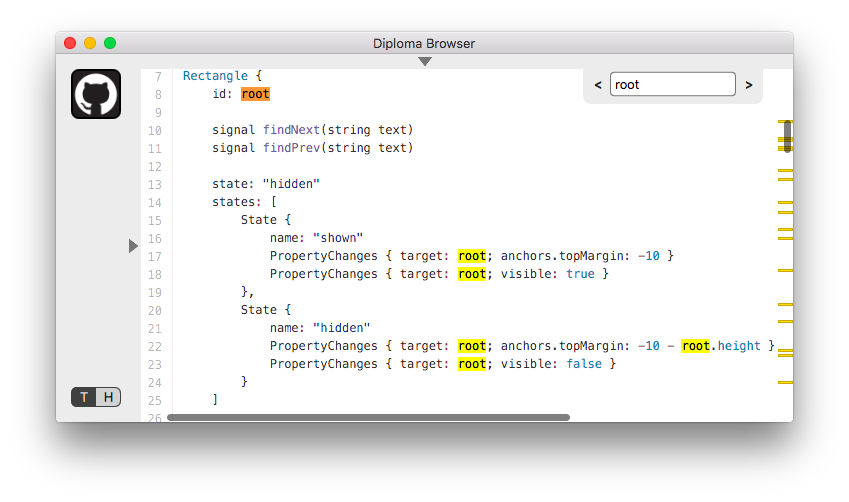
\includegraphics[scale=0.5]{FindBar-screen}
    \caption{
        \label{fig:find-bar-screen}
        Find Text funkció működés közben
    }
\end{figure}

\newpage
\subsection{Form Validation és Localization}
A Form Validation funkció használatához nincs szükség a példa böngészőalkalmazás bővítésére,
hiszen a megjelenítendő üzenetet tartalmazó szövegbuborék megvalósítása a Qt WebEngine modul
része, ami a megfelelő esemény hatására meg is jelenik. A funkció segítségével viszont jól
demonstrálható egy másik új funkció, a Localization. A Qt WebEngine Localization funkciója
miatt a Form Validation üzenetnek a Qt \texttt{QLocale} API-ján keresztül beállított nyelven
kell megjelenítenie.

A QML-ben nincs API a locale beállításához, viszont a nyelv kiegészíthető olyan C++ nyelven
megvalósított függvénnyel, ami elvégzi a beállítást:
\begin{lstlisting}[title=utils.h]
 class Utils : public QObject {
    Q_OBJECT
 public:
    Q_INVOKABLE static void setLocale(const QString &locale);
    /* ... */
 };

 inline void Utils::setLocale(const QString &locale)
 {
    QLocale::setDefault(QLocale(locale));
 }

 /* ... */
\end{lstlisting}
A \texttt{Utils} osztály már be van regisztrálva a QML környezetbe az alkalmazás fő belépési
pontjában (\texttt{main.cpp}). A \texttt{setLocale(locale)} függvény a \texttt{Q\_INVOKABLE}
makróval lett annotálva, ami lehetővé teszi, hogy QML-ből is hívható legyen. Az új függvény
segítségével az \texttt{appSettings}-ben tárolt nyelvi beállítással felüldefiniálhatjuk a
Qt alapértelmezett nyelvi beállításait az \texttt{ApplicationWindow} példány létrejöttekor:
\begin{lstlisting}[title=main.qml]
 ApplicationWindow {
    /* ... */

    Component.onCompleted: {
        utils.setLocale(appSettings.locale);
        viewListModel.create();
        viewListModel.select(viewListModel.count - 1);
    }
 }
\end{lstlisting}
Minden a locale inicializáció után létrejött \texttt{WebEngineView} példány a hozzátartozó
új Render Processt a \texttt{-{}-lang locale} kapcsolóval fogja indítani, ahol a
\texttt{locale} a \texttt{QLocale} API-n keresztül beállított nyelv. Az első
\texttt{WebEngineView} példány (tab) éppen ezért az inicializáció után van létrehozva:
\texttt{viewListModel.create();}

Célszerű lehet a nyelvi beállításokat futás közben is megváltoztatni, ezért a
\texttt{SettingsPanel} QML típus példánya tartalmaz egy lenyíló listát, ahol a támogatott
nyelvek közül lehet választani:
\begin{lstlisting}[title=main.qml]
ComboBox {
    id: localeCombo

    model: LocaleListModel { }
    textRole: "name"

    property string locale: appSettings.locale
    onCountChanged: currentIndex = model.findLocale(locale)
    onCurrentIndexChanged: localeCombo.locale =
                            model.get(currentIndex).locale
}
\end{lstlisting}
A támogatott nyelvek kézzel vannak hozzáadva a \texttt{LocaleListModel} QML típushoz, továbbá
ki vannak egészítve az a rendszer által használt nyelvvel, amit a Qt alapértelmezetten
használ. Mivel a \texttt{LocaleListModel} hamarabb van példányosítva, mint ahogy az
\texttt{ApplicationWindow} létrejön, ezért ezen a ponton még nincs felüldefiniálva a Qt
alapértelmezett nyelve. A lenyíló listában megjelenített neveket (\texttt{name} role) a
Qt API-n keresztül kérdezem le, így a \texttt{LocaleListModel} egyszerűen, akár dinamikusan
is bővíthető:
\newpage
\begin{lstlisting}[title=models/LocaleListModel.qml]
ListModel {
    id: root

    function addLocale(locale) {
        locale = locale.substring(0, 2);
        if (findLocale(locale) < 0) {
           append({ "locale": locale,
                    "name": Qt.locale(locale).nativeLanguageName
                  });
        }
    }

    /* ... */
    Component.onCompleted: {
        addLocale(Qt.locale().name);
        addLocale("en"); addLocale("de"); addLocale("hu");
    }
}
\end{lstlisting}

\begin{figure}[H]
    \centering
    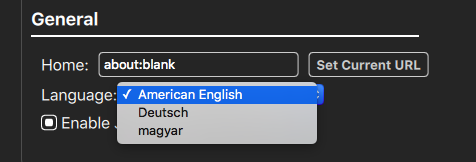
\includegraphics[scale=0.6]{locale-combo}
    \caption{
        \label{fig:locale-combo}
        Nyelvet kiválasztó lenyíló lista a \texttt{SettingsPanel}-en
    }
\end{figure}

\noindent
A nyelvi beállítás kiválasztás után nem lesz érvényes azonnal, azt a \texttt{SettingsPanel}
\textit{Ok} gombjának megnyomásával lehet alkalmazni (a \texttt{SettingsPanel} bezárása
visszavonja a nyelvi beállítást). Mivel új nyelvet beállítani a már futó Render Processekre
még nincs lehetőség, ezért az új nyelv beállítása után a böngészőalkalmazás felajánlja
(\texttt{SettingsPanel} confirm dialog), hogy újraindítja a tabokhoz tartozó már futó
processzeket, ami a böngészési előzmények elvesztésével jár:
\begin{lstlisting}[title=main.qml]
SettingsPanel {
    id: settingsPanel
    /* ... */

    onRestartRequest: {
        for (var i = 0; i < viewListModel.count; ++i)
            viewListModel.restart(i);
    }
}
\end{lstlisting}

Az előzmények elvesztésének, az az oka, hogy a processzek újraindítása a meglévő tabok
bezárásával és újra megnyitásával történik. A jelenlegi Qt WebEngine API-val csak az éppen
látható oldal URL-jének lementésére van lehetőség:
\begin{lstlisting}[title=models/WebEngineViewListModel.qml]
ListModel {
    id: root

    /* ... */

    function restart(index) {
        var currentIndex = wrapper.currentItem.index;
        var webEngineView = get(index).webEngineView;
        var url = webEngineView.url;

        close(index);
        create(index, url);

        if (index == currentIndex)
            select(index);

        webEngineView.destroy(1000);
    }
 }
\end{lstlisting}

A Form Validation funkcióval demonstrált eredmény az alábbi
(\ref{fig:validation-message-localization}) ábrán látható.

\begin{figure}[H]
    \centering
    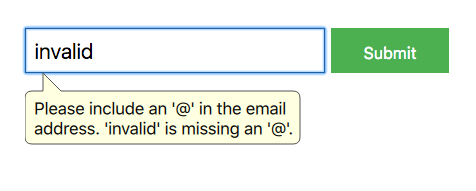
\includegraphics[scale=0.6]{validation-message-english}
    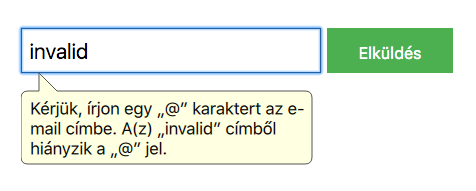
\includegraphics[scale=0.6]{validation-message-magyar}
    \caption{
        \label{fig:validation-message-localization}
        Form Validation angolul és magyarul
    }
\end{figure}


\addtocontents{toc}{\ }
\chapter*{Eredmények}
\addcontentsline{toc}{section}{Eredmények}

\enlargethispage{\baselineskip}

Dolgozatomban 8 db új QtWebEngine funkciót valósítottam meg és mutattam be. Ebből 4 db a
QtWebKitből átvett és továbbfejlesztett (Navigation History, Find Text, Authentication
Dialog, Favicon Manager), 1 db HTML5 funkció (Form Validation) és 3 db a hibakeresést és
tesztelést segíti (Log Level, Test Support API, Localization). A 8 db funkcióból 7 db
elérhető a Qt legfrissebb (5.6) stabil kiadásában. A Favicon Manager a készülő 5.7-es
verzióban biztosan benne lesz.

27 db patch-et nyújtottam be a Qt közösségnek, amelyek szorosan ezekhez a funkciókhoz
kapcsolódnak és be is kerültek a QtWebEngine kódjába. 1 db patch QtDeclarative komponensbe
került be, ami egy a Favicon Manager tesztelése közben felfedezett \texttt{Context2D}
QML típus hibáját javítja.

A dolgozatban bemutatott patcheken túl, még 35 db patchem került be (eddig összesen 62 db) a
QtWebEngine-be. Ezek a bemutatott funkciókhoz szorosan nem köthető, elsősorban hibajavítások,
új teszt esetek és karbantartási munkálatok. A javítások mindhárom legfontosabb desktop
platformra kiterjednek (GNU/Linux, Windows, OS X).

A munka során hivatalosan további 34 db patchet review-oltam, amelyből 8 db köthető a
bemutatott funkciókhoz. A dolgozathoz készített, QtWebEngine-re épülő példa
böngészőalkalmazás további ötleteket adott a funkciók tovább fejlesztésére (pl. Navigation
History kibővítése ikon támogatással), egyes részeit tervezem felhasználni a QtWebEngine-hez
hozzáadott példa alkalmazásokban és a funkciók teszteléséhez is hasznos volt.

\begin{figure}[H]
    \centering
    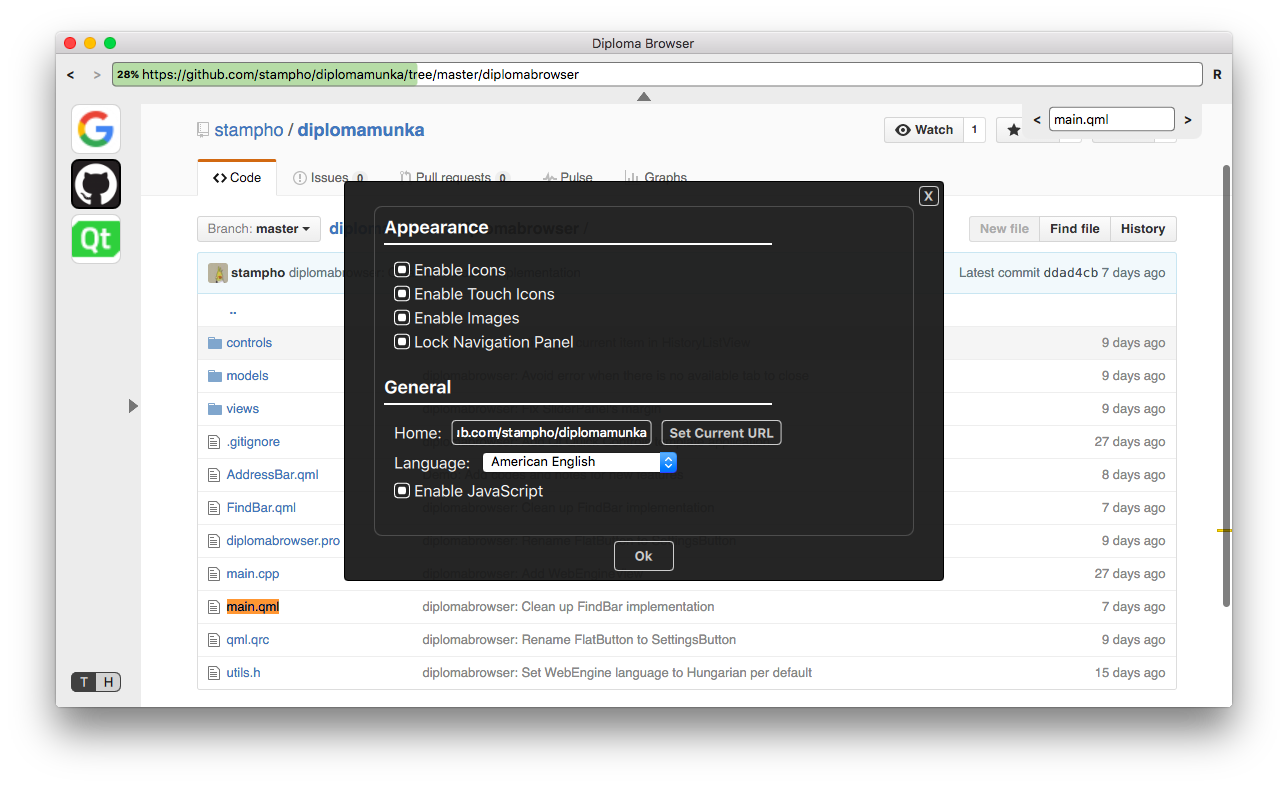
\includegraphics[scale=0.32]{diplomabrowser-result}
\end{figure}


%%% EPILOGUE %%%

\begin{thebibliography}{9}
    \addcontentsline{toc}{section}{Irodalomjegyzék}

    \bibitem{bib:qt-blog-introducing-qtwebengine}
        Qt Blog: Introducing the Qt WebEngine \\
        \href{http://blog.qt.io/blog/2013/09/12/introducing-the-qt-webengine/}
        {http://blog.qt.io/blog/2013/09/12/\\
        introducing-the-qt-webengine/}

    \bibitem{bib:wiki-chromium}
        Wikipedia: Chromium (web browser) \\
        \url{https://en.wikipedia.org/wiki/Chromium_(web_browser)}

    \bibitem{bib:wiki-chrome}
        Wikipedia: Google Chrome \\
        \url{https://en.wikipedia.org/wiki/Google_Chrome}

    \bibitem{bib:wiki-blink}
        Wikipedia: Blink (web engine) \\
        \url{https://en.wikipedia.org/wiki/Blink_(web_engine)}

    \bibitem{bib:chromium-displays-web-pages}
        Chromium: How Chromium Displays Web Pages \\
        \href{https://www.chromium.org/developers/design-documents/displaying-a-web-page-in-chrome}
        {https://www.chromium.org/developers/design-documents/\\
         displaying-a-web-page-in-chrome}

    \bibitem{bib:chromium-blink}
        Chromium: Blink \\
        \url{http://www.chromium.org/blink}

    \bibitem{bib:chromium-gpu}
        Chromium: GPU Accelerated Compositing in Chrome \\
        \href{https://www.chromium.org/developers/design-documents/gpu-accelerated-compositing-in-chrome}
        {https://www.chromium.org/developers/design-documents/\\
        gpu-accelerated-compositing-in-chrome}

    \bibitem{bib:chromium-oopifs}
        Chromium: Rendering and compositing out of process iframes \\
        \href{https://www.chromium.org/developers/design-documents/oop-iframes/oop-iframes-rendering}
        {https://www.chromium.org/developers/design-documents/\\
        oop-iframes/oop-iframes-rendering}

    \bibitem{bib:chromium-texture-mailbox}
        Chromium: CHROMIUM\_texture\_mailbox.txt \\
        \href{https://src.chromium.org/viewvc/chrome/trunk/src/gpu/GLES2/extensions/CHROMIUM/CHROMIUM_texture_mailbox.txt}
        {https://src.chromium.org/viewvc/chrome/trunk/src/gpu/\\
        GLES2/extensions/CHROMIUM/CHROMIUM\_texture\_mailbox.txt}

    \bibitem{bib:webkit-webkit2}
        WebKit: WebKit2 \\
        \url{https://trac.webkit.org/wiki/WebKit2}

    \bibitem{bib:chromium-multi-process}
        Chromium: Multi-process Architecture \\
        \href{https://www.chromium.org/developers/design-documents/multi-process-architecture}
        {https://www.chromium.org/developers/design-documents/\\
        multi-process-architecture}

    \bibitem{bib:chromium-blog-multi-process}
        Chromium Blog: Multi-process Architecture \\
        \href{http://blog.chromium.org/2008/09/multi-process-architecture.html}
        {http://blog.chromium.org/2008/09/\\
        multi-process-architecture.html}

    \bibitem{bib:chromium-process-models}
        Chromium: Process Models \\
        \href{https://www.chromium.org/developers/design-documents/process-models}
        {https://www.chromium.org/developers/design-documents/\\
        process-models}

    \bibitem{bib:chromium-plugins}
        Chromium: Plugin Architecture \\
        \href{https://www.chromium.org/developers/design-documents/plugin-architecture}
        {https://www.chromium.org/developers/design-documents/\\
        plugin-architecture}

    \bibitem{bib:chromium-content-module}
        Chromium: Content module \\
        \url{https://www.chromium.org/developers/content-module}

    \bibitem{bib:chromium-content-api}
        Chromium: Content API \\
        \href{https://www.chromium.org/developers/content-module/content-api}
        {https://www.chromium.org/developers/content-module/\\
        content-api}

    \bibitem{bib:qt-wiki-about-qt}
        Qt Wiki: About Qt \\
        \url{https://wiki.qt.io/About_Qt}

    \bibitem{bib:qt-wiki-qt-history}
        Qt Wiki: Qt History \\
        \url{https://wiki.qt.io/Qt_History}

    \bibitem{bib:qt-doc-webengine-overview}
        Qt Documentation: Qt WebEngine Overview \\
        \url{http://doc.qt.io/qt-5/qtwebengine-overview.html}

    \bibitem{bib:qt-about-us}
        The Qt Company: About Us \\
        \url{http://www.qt.io/about-us}

    \bibitem{bib:qt-doc-qtmodules}
        Qt Documentation: All Modules \\
        \url{http://doc.qt.io/qt-5/qtmodules.html}

    \bibitem{bib:qt-doc-qt-gui}
        Qt Documentation: Qt GUI \\
        \url{http://doc.qt.io/qt-5/qtgui-index.html}

    \bibitem{bib:qt-doc-user-interfaces}
        Qt Documentation: User Interfaces \\
        \url{http://doc.qt.io/qt-5/topics-ui.html}

    \bibitem{bib:qt-doc-qt-widgets}
        Qt Documentation: Qt Widgets \\
        \url{http://doc.qt.io/qt-5/qtwidgets-index.html}

    \bibitem{bib:qt-doc-qt-qml}
        Qt Documentation: Qt QML \\
        \url{http://doc.qt.io/qt-5/qtqml-index.html}

    \bibitem{bib:qt-doc-qt-quick}
        Qt Documentation: Qt Quick \\
        \url{http://doc.qt.io/qt-5/qtquick-index.html}

    \bibitem{bib:qt-doc-qt-quick-scene-graph}
        Qt Documentation: Qt Quick Scene Graph \\
        \href{http://doc.qt.io/qt-5/qtquick-visualcanvas-scenegraph.html}
        {http://doc.qt.io/qt-5/\\
        qtquick-visualcanvas-scenegraph.html}

    \bibitem{bib:qt-doc-qt-webview}
        Qt Documentation: Qt WebView \\
        \url{http://doc.qt.io/qt-5/qtwebview-index.html}

    \bibitem{bib:qt-doc-qt-websockets}
        Qt Documentation: Qt WebSockets \\
        \url{http://doc.qt.io/qt-5/qtwebsockets-index.html}

    \bibitem{bib:qt-doc-qt-webchannel}
        Qt Documentation: Qt WebChannel \\
        \url{http://doc.qt.io/qt-5/qtwebchannel-index.html}

    \bibitem{bib:kdab-qt-webchannel}
        KDAB: Qt WebChannel: bridging the gap between C++/QML and the web \\
        \href{https://www.kdab.com/qt-webchannel-bridging-gap-cqml-web}
        {https://www.kdab.com/\\
        qt-webchannel-bridging-gap-cqml-web}

    \bibitem{bib:qt-doc-qtwebengine-overview}
        Qt Documentation: Qt WebEngine Overview \\
        \url{http://doc.qt.io/qt-5/qtwebengine-overview.html}

    \bibitem{bib:qt-doc-qt-webengine-process}
        Qt Documentation: Qt WebEngine Process \\
        \href{http://doc.qt.io/qt-5/qtwebengine-overview.html\#qt-webengine-process}
        {http://doc.qt.io/qt-5/qtwebengine-overview.html\#\\
        qt-webengine-process}

    \bibitem{bib:qt-doc-qt-webengine-core}
        Qt Documentation: Qt WebEngine Core C++ Classes \\
        \url{http://doc.qt.io/qt-5/qtwebenginecore-module.html}

    \bibitem{bib:qt-wiki-d-pointer}
        Qt Wiki: D-Pointer \\
        \url{https://wiki.qt.io/D-Pointer}

    \bibitem{bib:qt-doc-qt-webengine-widgets}
        Qt Documentation: Qt WebEngine Widgets C++ Classes \\
        \url{http://doc.qt.io/qt-5/qtwebenginewidgets-module.html}

    \bibitem{bib:qt-doc-qt-webengine-quick}
        Qt Documentation: Qt WebEngine QML Types \\
        \url{http://doc.qt.io/qt-5/qtwebengine-qmlmodule.html}

\end{thebibliography}


\chapter*{Nyilatkozat}
\addcontentsline{toc}{section}{Nyilatkozat}

\noindent
Alulírott Varga Péter programtervező informatikus MSc szakos hallgató, kijelentem, hogy a
dolgozatomat a Szegedi Tudományegyetem, Informatikai Tanszékcsoport Szoftverfejlesztés
Tanszékén készítettem, programtervező informatikus MSc diploma megszerzése érdekében.

Kijelentem, hogy a dolgozatot más szakon korábban nem védtem meg, saját munkám eredménye
és csak hivatkozott forrásokat (szakirodalom eszközök, stb.) használtam fel.

Tudomásul veszem, hogy a diplomamunkámat a Szegedi Tudományegyetem Informatikai Tanszékcsoport
könyvtárában, a helyben olvasható könyvek között helyezik el.

\vspace*{2cm}

\begin{tabular}{lc}
    Szeged, \today \hspace{2cm} & \makebox[6cm]{\dotfill} \\
                                & aláírás
\end{tabular}


\chapter*{Köszönetnyílvánítás}
\addcontentsline{toc}{section}{Köszönetnyílvánítás}

\noindent
Szeretnék köszönetet mondani Dr. Kiss Ákos témavezetőmnek a téma kutatása alatt nyújtott
támogatásáért és a diplomamunkám megírásában nyújtott segítségéért.

Ezen kívül szeretnék köszönetet mondani a \textit{The Qt Company} és a
\textit{Szegedi Tudományegyetem Szoftverfejlesztés Tanszék} volt és jelenleg is a QtWebEngine
projekten dolgozó munkatársainak a beszélgetésekért és a közösségnek benyújtott munkám
ellenőrzéséért és befogadásáért.


\chapter*{Mellékletek}
\addcontentsline{toc}{section}{Mellékletek}

\noindent
DVD lemez mely tartalmazza:
\begin{itemize}
    \item \texttt{QtWebEngine} modul \texttt{Git} repository-ját
    \item A bemutatott funkciókat megvalósító patch-eket
    \item A példa böngészőalkalmazás forráskódját
\end{itemize}

\end{document}
